%\documentclass[10pt,twocolumn,twoside]{IEEEtran}
%\documentclass[draftclsnofoot,onecolumn,12pt]{IEEEtran}
%\documentclass[draftclsnofoot,onecolumn,11pt,peerreview]{IEEEtran}
\documentclass[12pt]{article}
\usepackage{fullpage}
\usepackage{pgfplots}
\usepackage{subfigure}
\usepackage{tikz}

\usepackage{makeidx}

\usepackage[cmex10]{amsmath}
\usepackage{amsthm,amssymb,mathrsfs}
\usepackage{graphicx}
\usepackage{url}
\usepackage{cite}
%\usepackage{apacite}
%\usepackage{natbib}
\usepackage{lineno}
\usepackage{verbatim}
\usepackage{bm}
\usepackage{multirow}
\usepackage{booktabs}
\usepackage{amsthm}
\usepackage{array}
%\usepackage[usenames,dvipsnames]{color}
\usepackage{color,xcolor}
\usepackage{framed}
\usepackage{hyperref}
\usepackage[titletoc,title]{appendix}
%\renewcommand{\appendixname}{Appendix}
\definecolor{shadecolor}{gray}{0.9}
\newcommand*{\vertbar}{\rule[-0.75ex]{0.25pt}{2.5ex}}
\newcommand*{\horzbar}{\rule[.5ex]{2.5ex}{0.25pt}}

\DeclareMathOperator{\len}{len}

\begin{document}
\title{Approach for the Quora Question Pairs Challenge}
\author{ YesOfCourse}
\maketitle

\abstract{In the Quora Question Pairs Challenge, we were asked to build a model to classify whether question pairs are duplicates or not (multiple versions of the same question). This documents describes our team's solution which can be divided into diffrent parts: Pre-processing, Feature Engineering, Modeling and Post-processing.}


\begin{comment}
\section*{Personal details}
\begin{itemize}
\item Team Name: Turing Test
\item Team Members: Chenglong Chen, Kostia
%\item Location: Shenzhen, Guangdong, China
\item Email: \url{c.chenglong@gmail.com}
\item Competition: \href{https://www.kaggle.com/c/home-depot-product-search-relevance}{Home Depot Product Search Relevance}
\end{itemize}
\end{comment}

\section*{Personal details}
\begin{itemize}
\item[] Team Name: \textbf{YesOfCourse}
\item[] Members:
\begin{itemize}
\item[$\bullet$] \textbf{Liang Pang} \\
%	 Location: Kyiv, Ukraine \\
	Email: \url{pangliang@gmail.com}
\item[$\bullet$] \textbf{Yixing Fan} \\
%	 Location: Kyiv, Ukraine \\
	Email: \url{fanyixing@gmail.com}
\item[$\bullet$] \textbf{Jianpeng Hou} \\
%	 Location: Shenzhen, Guangdong, China\\
	Email: \url{houjp1992@gmail.com}
\item[$\bullet$] \textbf{Xinyu Yue} \\
%	 Location: Shenzhen, Guangdong, China\\
	Email: \url{yuexinyu@gmail.com}
\item[$\bullet$] \textbf{Guocheng Niu} \\
%	 Location: Shenzhen, Guangdong, China\\
	Email: \url{niuox@gmail.com}
\end{itemize}
\item[] Competition: \href{https://www.kaggle.com/c/quora-question-pairs/}{Quora Question Pairs}
\end{itemize}

\newpage
\tableofcontents

\newpage


\section{Summary}

Our solution consisted of four main parts: Pre-processing, Feature Engineering, Modeling and Post-processing. What's more, we developed a light weight Machine Learning framework \textbf{FeatWheel} to help us to finish ML jobs, such as feature extraction, feature merging and so on.

In pre-processing, we process the text of data with text cleaning, word stemming, removing stop words and shared words and can form different versions of original data. In feature engineering, we extracted features based on various versions of data. The features can be classified in to three categories:Statistical Features, NLP Features and Graph Features. In modeling, we build deep models, boosting models (using XGBoost, LightGBM) and linear models (Linear Regression) and build a multi-layer stacking system to ensemble different models together. As we all know, the distribution of the training data and test data are quite different, so we made post-processing on the prediction results. We cut the data into different parts according to the clique size and rescale the results in different parts. 

\subsection{Flowchart}

The flowchart of our method is shown in Fig. \ref{fig:Flowchart}.

\begin{figure}[ht]
  \centering
  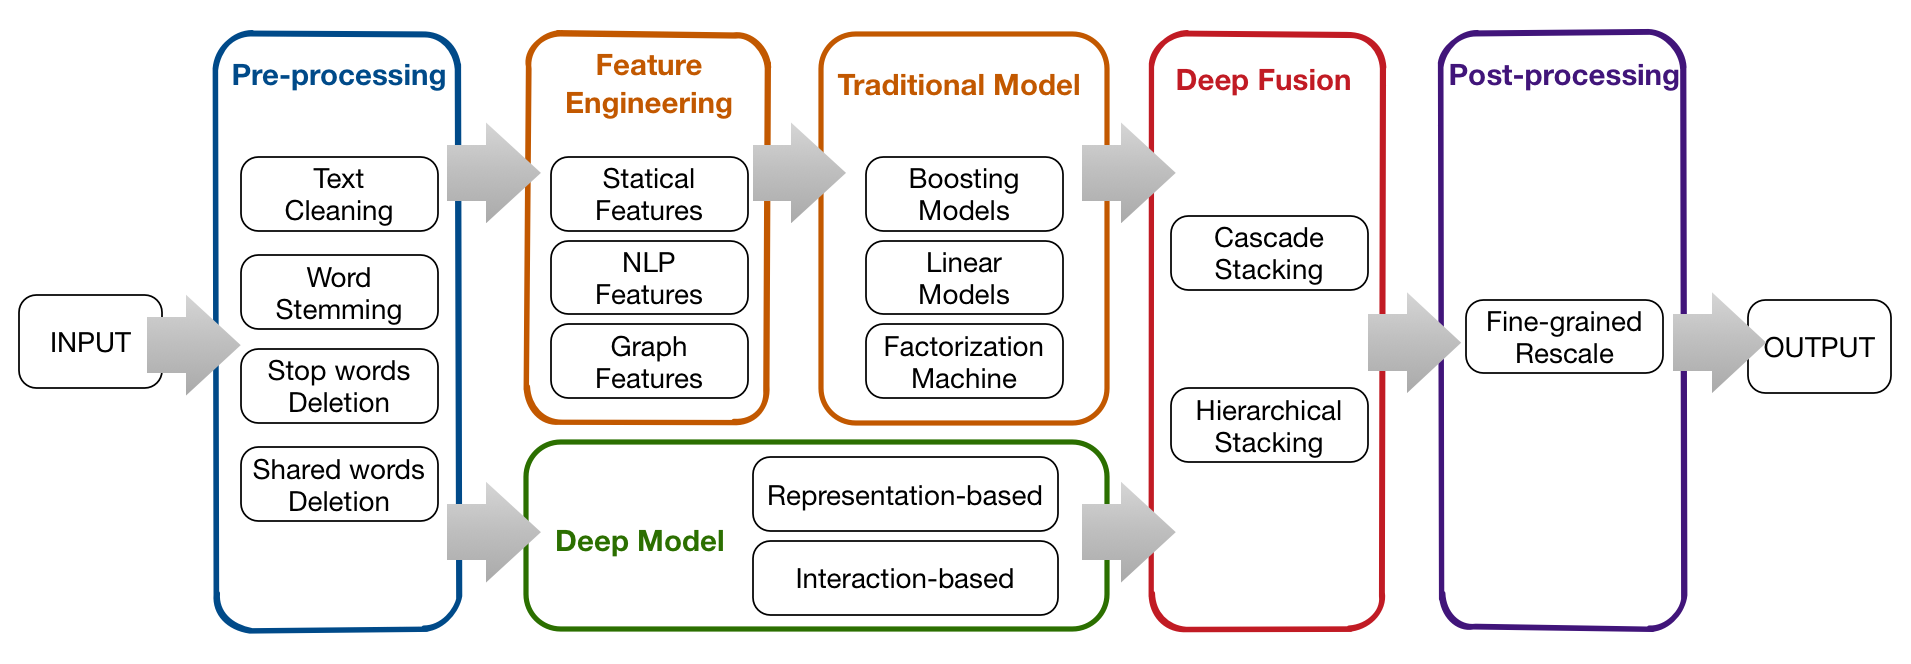
\includegraphics[width=0.9\textwidth]{../img/flowchart}\\
  \caption{The flowchart of our method.}
  \label{fig:Flowchart}
\end{figure}

\subsection{Submission}
\label{subsec:Results_description}

Submissions were evaluated on the log loss between the predicted values and the group truth. In specific, the best single model we have obtained during the competition was an XGBoost model with tree booster of Public LB score \textbf{0.12653} and Private LB score \textbf{0.13067} (without post-process). Our final submission was a stacking result of multiple models. This submission scored \textbf{0.11450} on Public LB and \textbf{0.11768} on Private LB (with post-process), ranking \textbf{4} out of \textbf{3396} teams.

\section{Pre-processing}


Pre-processing

\section{Feature Engineering}

Feature Engineering  

\section{Modeling}

Modeling

\section{Post-processing}

Post-processing

\section{ML Framework}

ML Framework

\section{Acknowledgement}

Acknowledgement

A few steps are applied to clean up the text. These steps were done separately by the two parts of our team. Unless otherwise noted, Igor\&Kostia's part is implemented in \texttt{homedepot\_functions.py} and  \texttt{text\_processing.py}. For Chenglong's part please see \texttt{data\_processor.py}.

\subsection{Initial steps}
They included making the text lowercase, replacement or cleaning of some symbols and some pattern replacement.
Some examples of the replacements are shown in the table below:

\begin{tabular}{|c|c|}
  \hline
  Symbol & Replacement \\ \hline
  \&amp; & \& \\ \hline
 \&nbsp; &  \\ \hline
  ; & . \\ \hline
: & . \\ \hline
+ &  \\ \hline
* &  x \\ \hline
\end{tabular}

Other text cleaning included:
\begin{itemize}
\item Removed words in parentheses or replace parentheses with dots.
\item Removed commas between digits (for example, $10,000$ was replaced with $10000$).
\item Added dot and space between a digit (left) and a letter (right).
\item Added space between at least three letters (left) and a digit (right).
\item Replaced  $\backslash$ or / between letters with a space.
\end{itemize}

The punctuation was important for extraction of the most important words from the text or tagging words using \emph{NLTK.pos\_tagger()} function. Otherwise, it was removed at all.

We also noticed that product description is produced by concatenation of text lines, so that some words have capital letters in the middle (like \emph{firstSecond}). We added a space in such words, but only in those that are not found in product title. So, we would transform the string \emph{firstSecond} to \emph{first Second}, but leave \emph{InSinkErator} as it is.

\subsection{Spell Correction}
It is mostly done for search term which contains many spelling errors.
\begin{itemize}
\item Replacement of search terms using \textbf{the Google dictionary} from the forum  \cite{Google_dict}.
\item \textbf{Manual replacements} posted on the forum.
\item \textbf{Automatic spell checker} (Igor\&Kostia). It is implemented in \texttt{text\_processing.py}. It tries to find replacement for words from search term which are not found in product title (in this paragraph we name them \emph{'misspelled'} words). First, the algorithm checks whether the misspelled word is actually a combination of two separate words. Second, it searches for a good replacement in product titles that are matched to queries with the misspelled words. Finally, all product title is used as a vocabulary to find an appropriate replacement.
\end{itemize}


\subsection{Concatenation of Numbers with Measure Units}
This part is best illustrated by the following code:

\begin{verbatim}
s = re.sub('(?<=[0-9])[\ ]*pound[s]*(?=\ |$|\.)', '-lb ', s)
s = re.sub('(?<=[0-9])[\ ]*lb[s]*(?=\ |$|\.)', '-lb ', s)
s = re.sub('(?<=[0-9])[\ ]*gallon[s]*(?=\ |$|\.)', '-gal ', s)
s = re.sub('(?<=[0-9])[\ ]*gal(?=\ |$|\.)', '-gal ', s)
\end{verbatim}


\subsection{Thesaurus Replacement}
In total, we made about 200 replacements that might be described as follows:

\begin{itemize}
\item \textbf{'Stemming':} \emph{winterizing}	$\rightarrow$ \emph{winterizer}.
\item \textbf{Synonym replacement:} \emph{lamp}	$\rightarrow$ \emph{light}.
\item \textbf{Abbreviation convertion:} \emph{bbq}	$\rightarrow$ \emph{barbeque}.
\item \textbf{Uniform spelling.} Many words can be spelled differently in the dataset: \emph{mail box} and \emph{mailbox}, \emph{fibre} and \emph{fiber}, \emph{chain saw} and \emph{chainsaw}, \emph{aluminium} and \emph{aluminum}. We made the spelling of some of such words uniform throughout all text columns.
\item \textbf{Brands and materials:} \emph{lg electronics} $\rightarrow$    \emph{lg} and  \emph{medium density fiberboard}  $\rightarrow$  \emph{mdf}
\end{itemize}



\subsection{Part-of-Speech Tagging}
It was done by \emph{NLTK.pos\_tagger()} function.

\subsection{Extracting information about brands and materials}
We used appropriate rows from file \texttt{attributes.csv}. Then we extracted brand and materials from the available docs (search term, product title, product description, attribute bullets). Later we will use these docs with or without brand/material information to generate different sets of features.

It should be noted that some 'true brand names' are long: for example, \emph{'BEHR Premium Plus'}. But it is likely to be as simple as 'BEHR' in the query. So, once we found such a long brand name within a doc, we would replace it with a shorter version. In total, we replace 131 such long brand names.

\subsection{Dealing with Different Parts of Query or Product Title}
We noticed a structure in product title which helped us to find the most important part of the document. For example, in product title \emph{'Husky 52 in. 10-Drawer Mobile Workbench with Solid Wood Top, Black'} the product is workbench, not wood top. To deal with multiple patterns present in product title, we had to elaborate a complex algorithm, which extracted important words.

We also extracted the top trigram \cite{crowdflower_3place}. Igor and Kostia started this work independently, so in their notation the trigrams words are denoted as (\emph{before2thekey}, \emph{beforethekey}, \emph{thekey}), where \emph{thekey} is the last word in the trigram.

We separately dealt with text after words \emph{with}, \emph{for}, \emph{in}, \emph{without}.

\subsection{Final Steps}
To generate the most of the features we used stemmed text as an input.

\subsection{Other}
These part describes some of the processing done on Chenglong's side. Most of the processing are similar as Igor\&Kostia's, including lower case conversion, unit conversion, removing comma between digits, manual word replacement, google spelling correction, lemmatizing, stemming etc. However, they are done in different way, which is helpful for introducing diversity. In addition, we would like to mention a few words about the following parts.
\subsubsection{Splitting Lower Case Words and Upper Case Words}
In the production\_description, there are words concatenated without spacing. For example,
\begin{itemize}
\item hidden from \emph{viewDurable} rich \emph{finishLimited} lifetime \emph{warrantyEncapsulated} panels
\item Dickies quality has been built into every \emph{product.Excellent} \emph{visibilityDurable}.
\end{itemize}
This might due to that while creating the product description file, someone concatenated all the lines in a description file without adding spaces in between. To deal with such cases, we split the `lower[.?!]UPPER' pattern. For the above two examples, they become
\begin{itemize}
\item hidden from \emph{view Durable} rich \emph{finish Limited} lifetime \emph{warranty Encapsulated} panels
\item Dickies quality has been built into every \emph{product. Excellent} \emph{visibility Durable}.
\end{itemize}

\subsubsection{Mapping English Number to Digit}
We map English numbers, e.g., ``one'' and ``two'' to 1 and 2.

\subsubsection{Extracting Product Name}
We extract product name from both search\_term and product\_title using a similar method described in the 3rd place solution for CrowdFlower competition\cite{crowdflower_3place}.

\subsubsection{Home-made Spelling Checker}
We have built our own home-made spelling checker, which is inspired by Peter Norvig's post\cite{PeterNorvig}. Though not used in the final submission, it also helps to identify possible misspellings. Please see \texttt{PeterNovigSpellingChecker} and \texttt{AutoSpellingChecker} classes in \texttt{spelling\_checker.py} for details. Following is some of the output
\begin{verbatim}
 Run AutoSpellingChecker at search_term
 Building word corpus
 Building error correction pairs
 Building query correction map
                 original query 	                corrected query
                     linen tile 	                     liner tile
   ekena millwork cherry corbel 	     ekena millwork cherry core
     potting soil chemical free 	     potting pool chemical free
        ge dishwasher stainless 	         ge dishwasherstainless
    led shop light makita light 	    led shop light making light
     500 ft. thhn stranded blue 	     500 ft. thwn stranded bare
  roman shade cord idler pulley 	  roman shade come idler pulley
               gold panning pan 	               gold hanging pan
             green quadrato pot 	               green quadro pot
\end{verbatim}

\section{Feature Extraction}
\subsection{Chenglong's Part}
\label{subsec:FeatureExtraction_Chenglong}
As in CrowdFlower, we have many pairwise features that measures the similarity/distance between search\_term and product\_title, or search\_term and product\_description. So we implement a base class \texttt{BaseEstimator} that takes an \texttt{obs} (e.g., search\_term) and \texttt{target} (e.g., product\_title) as input. For some features, e.g., intersected position in CrowdFlower or ngram level similarity/distance, we need to use various aggregation methods to generate statistics such as max and mean.\footnote{For some features, we also use double aggregation.} \texttt{BaseEstimator} also serves this purpose. Most of our feature generators are based on \texttt{BaseEstimator}.

On the top, we have \texttt{StandaloneFeatureWrapper} and \texttt{PairwiseFeatureWrapper} for generating standalone features and pairwise features respectively, using various feature generators, between various \texttt{obs} and \texttt{target} (e.g., search\_term vs. product\_title and search\_term vs. product\_description). Please find details for these classes in the module \texttt{feature\_base}.

All the similarity/distance measurements are in the module \texttt{./utils/dist\_utils}.

\subsubsection{Basic Features}
\label{subsec:Basic_Features}
We generated some basic descriptive features with file \texttt{feature\_basic.py}.
\begin{itemize}
\item \textbf{DocId}: numerical encoding of \texttt{obs} (e.g., search\_term, product\_title; only used with tree model)
\item \textbf{DocIdOneHot}: onehot encoding of \texttt{obs} (e.g., search\_term, product\_title; only used with linear model)
\item \textbf{DocIdEcho}: return the original Id of \texttt{obs}; this is only for product\_uid
\item \textbf{ProductUidDummy1}: dummy 1 for product\_uid
\item \textbf{ProductUidDummy2}: dummy 2 for product\_uid
\item \textbf{ProductUidDummy3}: dummy 3 for product\_uid
\item \textbf{DocLen}: length of \texttt{obs}
\item \textbf{DocFreq}: frequency of \texttt{obs} in the corpus
\item \textbf{DocEntropy}: entropy of \texttt{obs}
\item \textbf{DigitCount}: count of digit in \texttt{obs}
\item \textbf{DigitRatio}: ratio of digit in \texttt{obs}
\item \textbf{UniqueCount\_Ngram}: count of unique word ngram in \texttt{obs}
\item \textbf{UniqueRatio\_Ngram}: ratio of unique word ngram in \texttt{obs}
\item \textbf{AttrCount}: count of attributes in product\_attribute\_list
\item \textbf{AttrBulletCount}: count of bullet attributes in product\_attribute\_list
\item \textbf{AttrBulletRatio}: ratio of bullet attributes in product\_attribute\_list
\item \textbf{AttrNonBulletCount}: count of non-bullet attributes in product\_attribute\_list
\item \textbf{AttrNonBulletRatio}: ratio of non-bullet attributes in product\_attribute\_list
\item \textbf{AttrHasProductHeight}: whether or not contains product height in product\_attribute\_list
\item \textbf{AttrHasProductWidth}: whether or not contains product width in product\_attribute\_list
\item \textbf{AttrHasProductLength}: whether or not contains product length in product\_attribute\_list
\item \textbf{AttrHasProductDepth}: whether or not contains product depth in product\_attribute\_list
\item \textbf{AttrHasIndoorOutdoor}: whether or not contains indoor/outdoor info in product\_attribute\_list
\end{itemize}

For using with linear model, we apply \texttt{np.log1p} to some of the above features, e.g., \texttt{DocLen} and \texttt{DocFreq} etc.

\subsubsection{Distance Features}
\label{subsec:Distance_Features}
We generated the following features with file \texttt{feature\_distance.py}.
\begin{itemize}
\item \textbf{JaccardCoef\_Ngram}: jaccard coefficient of \texttt{obs} word ngram and \texttt{target} word ngram
\item \textbf{DiceDistance\_Ngram}: same as above but using dice distance
\item \textbf{CompressionDistance}: compression distance between \texttt{obs} and \texttt{target} (document level)
\item \textbf{EditDistance}: edit distance between \texttt{obs} and \texttt{target} (document level)
\item \textbf{EditDistance\_Ngram}: same as above, but in word ngram level with \textcolor{red}{double aggregation}. To see what double aggregation means, we take for example the feature:  \texttt{EditDistance\_Bigram\_Max\_Min\_search\_term\_x\_product\_title}. It means: for each word bigram in search\_term, compute the maximum value of the edit distance between this bigram and every word bigram in product\_title; then take the minimum value of those maximum values as output feature. \emph{Double aggregation allows to capture the similarity between \texttt{obs} and \texttt{target} (e.g., search\_term and product\_title) in word level.}
\end{itemize}

\subsubsection{Doc2Vec Features}
We generated the following features using file \texttt{feature\_doc2vec.py}.
\begin{itemize}
\item \textbf{Doc2Vec\_Vector}: doc2vec vector of \texttt{obs} (not used in final submission)
\item \textbf{Doc2Vec\_Vdiff}: difference between doc2vec vector of \texttt{obs} and doc2vec vector of \texttt{target} (not used in final submission)
\item \textbf{Doc2Vec\_CosineSim}: cosine similarity between doc2vec vector of \texttt{obs} and doc2vec vector of \texttt{target}
\item \textbf{Doc2Vec\_RMSE}: RMSE between doc2vec vector of \texttt{obs} and doc2vec vector of \texttt{target}
\end{itemize}

Doc2Vec model are trained using \texttt{embedding\_trainer.py} with the provided data, i.e., search\_term, product\_title, product\_description, and product\_attribute.

\subsubsection{First and Last Ngram Features}
\label{subsubsec:Feature:Chenglong:First_Last_Ngram}
We generated the following features using file \texttt{feature\_first\_last\_ngram.py}.
\begin{itemize}
\item \textbf{FirstIntersectCount\_Ngram}: how many word ngram in \texttt{target} \textcolor{red}{closely matches} with the first ngram of \texttt{obs}. We choose \textcolor{red}{closely match} instead of \textcolor{blue}{exactly match} in the consideration of that there might be some misspelling characters in the word, e.g,. \emph{conditionar} (which should probably be \emph{conditioner}). The closeness is measured with edit distance.
\item \textbf{LastIntersectCount\_Ngram}: same as \textbf{FirstIntersectCount\_Ngram} but considering last ngram of \texttt{obs}
\item \textbf{FirstIntersectRatio\_Ngram}: same as \textbf{FirstIntersectCount\_Ngram} but normalized with the number of word ngram in \texttt{target}
\item \textbf{LastIntersectRatio\_Ngram}: same as \textbf{LastIntersectCount\_Ngram} but normalized with the number of word ngram in \texttt{target}
\end{itemize}
Compared to the \textbf{Intersect Count Features} described below, such features are designed to give more weight on the first and last ngram. One a more general level, one can add weighting according to the position of the word ngram in the search\_term or product\_title.

\subsubsection{Group Relevance Based Distance Features}
\label{subsubsec:Feature_Chenglong_Group_Dist}
We generated the following features using file \texttt{feature\_group\_distance.py}.
\begin{itemize}
\item \textbf{GroupRelevance\_Ngram\_Jaccard}: group by (search\_term, relevance) based distance features; (single) aggregation with various methods, e.g., max and mean etc. (see Sec 3.2.2 in Chenglong's Solution of CrowdFlower for details).
\end{itemize}
However, such features are NOT used in the final submission as we haven't achieved much improvement with these features. In CrowdFlower (where such features are reported with success in the 1st and 3rd solutions), there are about 260 unique queries and for each query and relevance combination, there are enough samples to obtain a reliable group based distance. However, in this competition, there are approximately 7.5 samples for each search\_term. Considering that there are 7 major relevance levels, there is not enough samples for such group based distance. This might be the reason why such features fail to work here. A possible way out would be to cluster similar search\_term first. For example, \emph{furnace air filters} and \emph{furnace filters with sensor} might be considered as within the same group/cluster.

\subsubsection{Group Relevance Features}
We generated the following features using file \texttt{feature\_group\_relevance.py}.
\begin{itemize}
\item \textbf{GroupRelevance}: group by search\_term/product\_title and compute some statistics (e.g., max and mean) of the relevance in the group.
\end{itemize}
However, such features are currently NOT used in model building due to similar reason mentioned in Sec. \ref{subsubsec:Feature_Chenglong_Group_Dist}.

\subsubsection{Intersect Count Features}
We generated the following features using file \texttt{feature\_intersect\_count.py}.
\begin{itemize}
\item \textbf{IntersectCount\_Ngram}: count of word ngram of \texttt{obs} that \textcolor{red}{closely matches} any word ngram of \texttt{target}.
\item \textbf{IntersectRatio\_Ngram}: same as \textbf{IntersectCount\_Ngram} but normalized with the total number of word ngram in \texttt{obs}
\item \textbf{CooccurrenceCount\_Ngram}: count of \textcolor{red}{closely matching} word ngram pairs between \texttt{obs} and \texttt{target}.
\item \textbf{CooccurrenceRatio\_Ngram}: same as \textbf{CooccurrenceCount\_Ngram} but normalized with the total number of word ngram pairs between \texttt{obs} and \texttt{target}.
\end{itemize}
As mentioned in Sec. \ref{subsubsec:Feature:Chenglong:First_Last_Ngram}, you can weight such feature according to the position of the word ngram in the search\_term or product\_title, besides extracting the intersect position as features as described in the following section.

\subsubsection{Intersect Position Features}
We generated the following features using file \texttt{feature\_intersect\_position.py}.
\begin{itemize}
\item \textbf{IntersectPosition\_Ngram}: see Sec 3.1.3 in Chenglong's Solution of CrowdFlower for details
\item \textbf{IntersectNormPosition\_Ngram}: see Sec 3.1.3 in Chenglong's Solution of CrowdFlower\cite{CrowdFlower_1st} for details
\end{itemize}

\subsubsection{Match Features}
We generated the following features using file \texttt{feature\_match.py}.
\begin{itemize}
\item \textbf{MatchQueryCount}: count of search\_term that occurs in \texttt{target}
\item \textbf{MatchQueryRatio}: same as \textbf{MatchQueryCount} but normalized with the length of \texttt{target}
\item \textbf{LongestMatchSize}: longest match size between \texttt{obs} and \texttt{target}
\item \textbf{LongestMatchRatio}: same as \textbf{LongestMatchSize} but normalized with the minimum length of \texttt{obs} and \texttt{target}
\item \textbf{MatchAttrCount}: count of attribute in product\_attribute\_list that matches search\_term
\item \textbf{MatchAttrRatio}: ratio of attribute in product\_attribute\_list that matches search\_term
\item \textbf{IsIndoorOutdoorMatch}: whether the indoor/outdoor info in seach\_term and product\_attribute\_list match
\end{itemize}

\subsubsection{Query Quality Features}
We generated the following features using file \texttt{feature\_query\_quality.py}.
\begin{itemize}
\item \textbf{QueryQuality}: measures the quality of search\_term using the edit distance among various versions, e.g., original search\_term and cleaned search\_term.
\item \textbf{IsInGoogleDict}: whether the search\_term is in the Google spelling correction dictionary or not.
\end{itemize}

\subsubsection{Statistical Cooccurrence TFIDF Features}
We generated the following features using file \texttt{feature\_tfidf.py}.
\begin{itemize}
\item \textbf{StatCoocTF\_Ngram}: for each word ngram in \texttt{obs}, count how many word ngram in \texttt{target} that \textcolor{red}{closely matches} it and then aggregate to obtain various statistics, e.g., max and mean.
\item \textbf{StatCoocTFIDF\_Ngram}: same as \textbf{StatCoocTF\_Ngram} but weight the count with IDF of the word ngram in the \texttt{obs} corpus
\item \textbf{StatCoocBM25\_Ngram}: same as \textbf{StatCoocTFIDF\_Ngram} but with BM25 weighting
\end{itemize}
All the feature above used \textcolor{red}{closely matching}.

\subsubsection{Vector Space Features}
We generated the following features using file \texttt{feature\_vector\_space.py}.
\begin{itemize}
\item \textbf{LSA\_Word\_Ngram}: LSA of \texttt{obs} word ngram
\item \textbf{LSA\_Char\_Ngram}: LSA of \texttt{obs} char ngram
\item \textbf{LSA\_Word\_Ngram\_Cooc}: LSA of cooccurrence word ngram between \texttt{obs} and \texttt{target}; see Sec. 3.3.2 in Chenglong's Solution of CrowdFlower\cite{CrowdFlower_1st} for how we generate cooccurrence terms.
\item \textbf{LSA\_Word\_Ngram\_Pair}: LSA after concatenating TFIDF of \texttt{obs} word ngram and TFIDF of \texttt{target} word ngram
\item \textbf{LSA\_Word\_Ngram\_CosineSim}: cosine similarity between LSA of \texttt{obs} word ngram and LSA of \texttt{target} word ngram
\item \textbf{LSA\_Char\_Ngram\_CosineSim}: same as \textbf{LSA\_Word\_Ngram\_CosineSim} but for char ngram
\item \textbf{TFIDF\_Word\_Ngram\_CosineSim}: same as \textbf{LSA\_Word\_Ngram\_CosineSim} but use TFIDF instead of LSA
\item \textbf{TFIDF\_Char\_Ngram\_CosineSim}: same as \textbf{LSA\_Word\_Ngram\_CosineSim} but use TFIDF instead of
\item \textbf{TSNE\_LSA\_Word\_Ngram\_Cooc}: 2-D TSNE of \textbf{LSA\_Word\_Ngram\_Cooc}
\item \textbf{TSNE\_LSA\_Word\_Ngram\_Pair}: 2-D TSNE of \textbf{LSA\_Word\_Ngram\_Pair}
\item \textbf{CharDistribution\_Ratio}: ratio between the char distribution of \texttt{obs} and char distribution of \texttt{target}
\item \textbf{CharDistribution\_CosineSim}: same as \textbf{CharDistribution\_Ratio} but use cosine similarity as similarity measurement
\item \textbf{CharDistribution\_KL}: same as \textbf{CharDistribution\_Ratio} but use KL divergence as distance measurement
\end{itemize}

\subsubsection{Word2Vec Features}
We generated the following features using file \texttt{feature\_word2vec.py}.
\begin{itemize}
\item \textbf{Word2Vec\_N\_Similarity}: n\_similarity between \texttt{obs} and \texttt{target}
\item \textbf{Word2Vec\_Centroid\_RMSE}: RMSE between the centroid vector of \texttt{obs} and centroid vector of \texttt{target}
\item \textbf{Word2Vec\_CosineSim}: \textcolor{red}{double aggregation} features. Take for example the feature \texttt{Word2Vec\_CosineSim\_Max\_Min\_search\_term\_x\_product\_title}. It means: for each word in search\_term, compute the maximum value of the cosine similarity between this word and every word in product\_title; then take the minimum value of those maximum values as output feature.
\end{itemize}
Word2Vec model are trained using \texttt{embedding\_trainer.py} with the provided data, i.e., search\_term, product\_title, product\_description, and product\_attribute. We also use pretrained models trained with Google News corpus and Wikipedia corpus as listed \href{https://github.com/3Top/word2vec-api}{here}.

\subsubsection{WordNet Similarity Features}
\label{subsec:wordnet}
We generated the following features using file \texttt{feature\_wordnet\_similarity.py}.
\begin{itemize}
\item \textbf{WordNet\_Path\_Similarity}: \textcolor{red}{double aggregation} features. Take for example the feature \texttt{WordNet\_Path\_Similarity\_Max\_Min\_search\_term\_x\_product\_title}. It means: for each word in search\_term, compute the maximum value of the \textcolor{blue}{similarity} between this word and every word in product\_title; then take the minimum value of those maximum values as output feature. The \textcolor{blue}{similarity} between two words is measured as following: for each word, we first obtain all its synset set then compute the maximum \texttt{path\_similarity} between these synset sets.
\item \textbf{WordNet\_Lch\_Similarity}: same as \textbf{WordNet\_Path\_Similarity} but use \texttt{lch\_similarity} instead of \texttt{path\_similarity}
\item \textbf{WordNet\_Wup\_Similarity}: same as \textbf{WordNet\_Path\_Similarity} but use \texttt{wup\_similarity} instead of \texttt{path\_similarity}
\end{itemize}
Such features are quite time consuming. A possible way to reduce the computation time would be to only consider those \emph{important word ngrams} as described in Igor\&Kostia's part, i.e., Sec. \ref{subsubsec:wordnet_IandK}.

\subsubsection{Feature Correlation with Target}
Fig. \ref{Fig:feature_corr_Chenglong} shows the correlation coefficients of our features with target relevance for each feature group. As shown, most of our feature groups exhibit high correlation with the target relevance indicating strong predictive power. Three feature groups, i.g., \texttt{edit\_distance}, \texttt{intersect\_count}, and \texttt{word2vec\_homedepot}, contain features with absolute correlation coefficient around 0.39. For the \texttt{word2vec} feature group, we have observed that features generated using model trained with Homedepot provided data exhibits higher correlation with the target, than those extracted with pre-trained Google News model and Wikipedia model.

\begin{figure}[t]
  \centering
  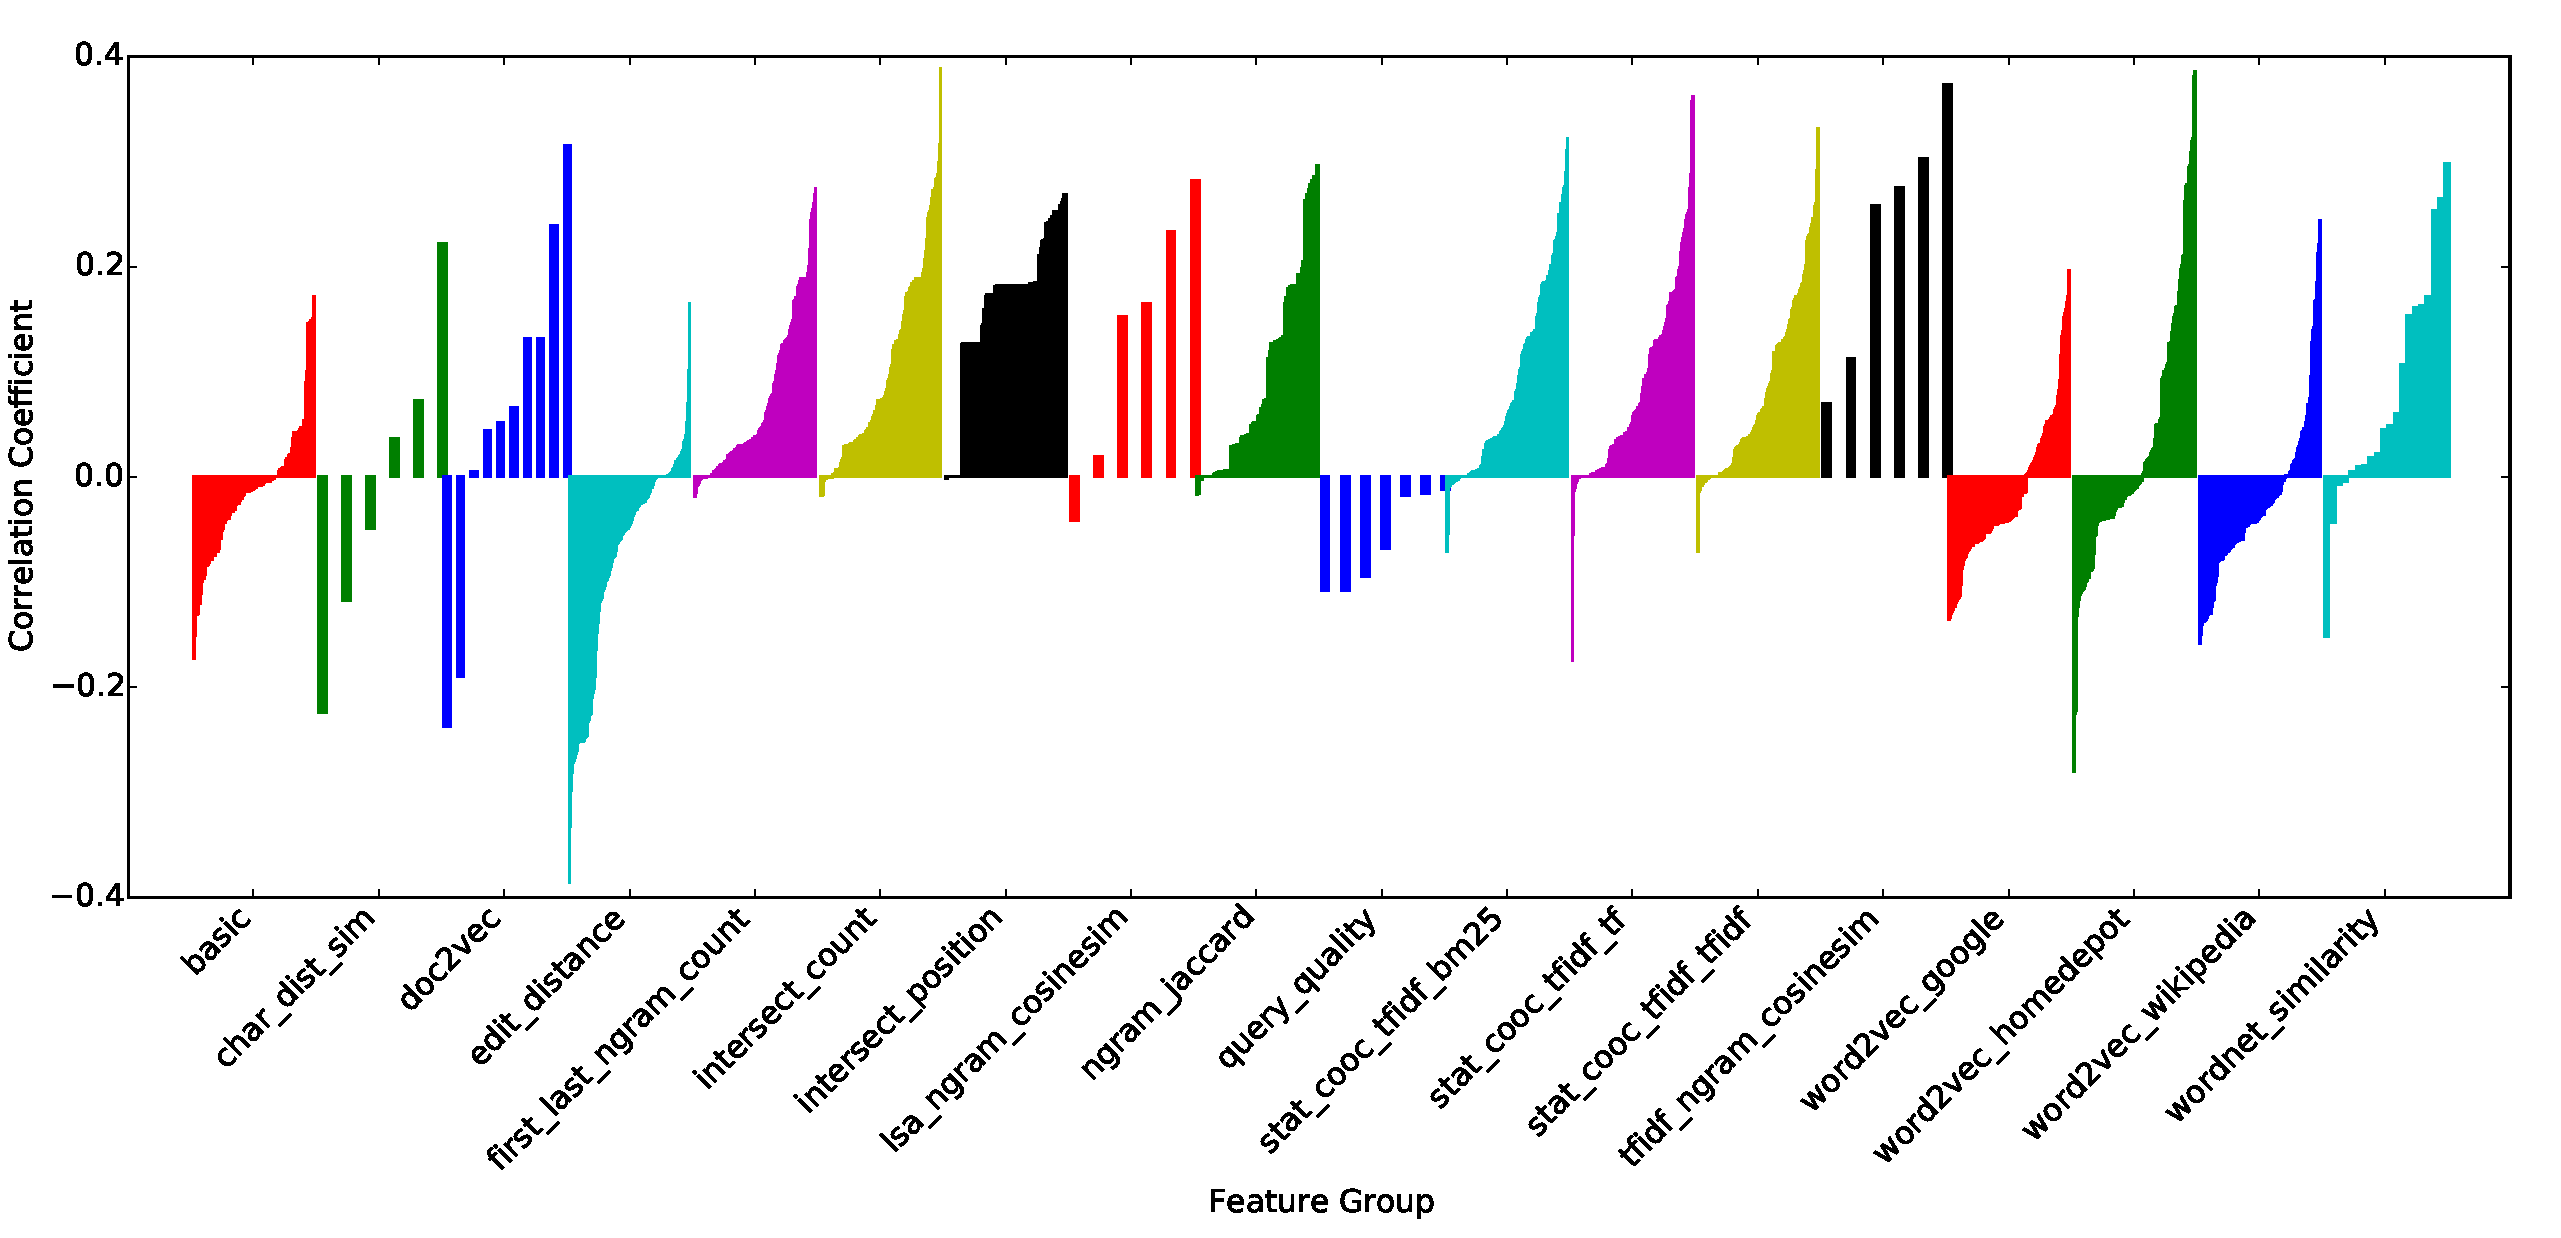
\includegraphics[width=1\textwidth]{../Fig/feature_corr_Chenglong.pdf}\\
  \caption{Correlation coefficients of Chenglong's features with target relevance for each feature group.}
  \label{Fig:feature_corr_Chenglong}
\end{figure}

\subsection{Igor\&Kostia's Part}
\label{subsec:Features_IandK}
Unless otherwise noted, the feature generation is done in file \texttt{feature\_extraction1.py}. Feature importances of 20 top features for our benchmark GradientBoostingRegressor model are shown in Fig.\ \ref{Fig:feature_importance_IandK}.

\begin{figure}
  \centering
  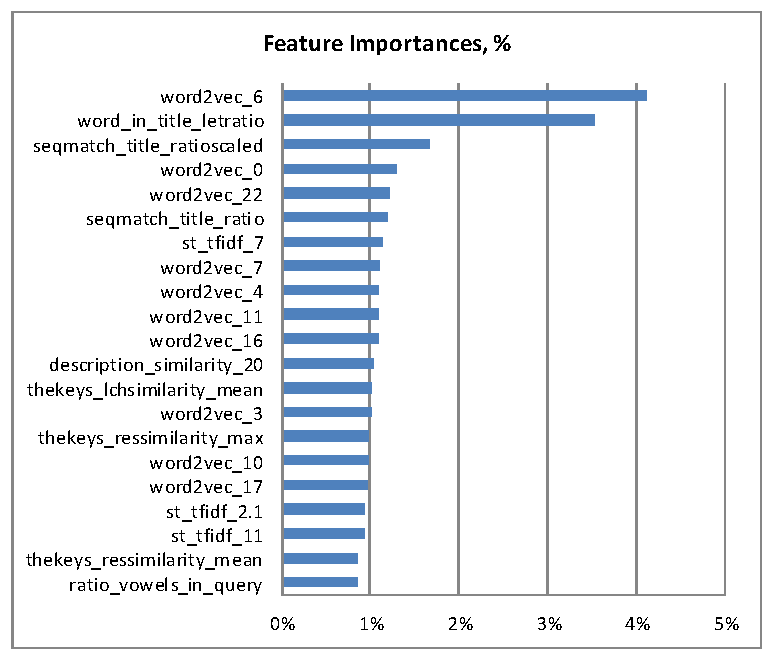
\includegraphics[width=0.7\textwidth]{../Fig/plot_feature_importances_benchmark.pdf}\\
  \caption{Feature importances of top 20 features for benchmark GradientBoostingRegressor model (Igor\&Kostia).}
  \label{Fig:feature_importance_IandK}
Note: \textbf{word2vec\_6} was calculated as \emph{n\_similarity()} between stemmed search term and stemmed product title.
\end{figure}

\subsubsection{Basic Features}
\label{subsubsec:Basic_Features_IandK}
\begin{itemize}
\item \textbf{len\_of\_\emph{strings}}: number of words in different available strings (e.g. search term, search term without brand, search terms without brand and material, brands/materials in search terms, words with digits in search term, the most important words in search term, nouns/verbs/adjectives in search terms, words after \emph{'for'} and \emph{'with'} in search terms and after \emph{'without'} in product titles, and similar variables for product title, product descriptions, product attributes etc.)
\item \textbf{size\_of\_brand/material\_in\_\emph{strings}}: number of distinct brands and materials in search term, product title, product description, attribute bullets.
\item \textbf{perc\_digits\_in\_\emph{strings}}: percentage of digits in different text variables.
\item \textbf{has\_attributes\_dummy}.
\item \textbf{no\_bullets\_dummy}.
\end{itemize}

The following three variables, which were inspired by \cite{dato:beatthebenchmark}, are also used to measure the 'amount' of information in the search term:
\begin{itemize}
\item \textbf{Ratio of meaningful words in search term}: the word is meaningful if WordNet knows synsets for the word.
\item \textbf{Average length of word in search term}.
\item \textbf{Ratio of vowels in search terms}.
\end{itemize}

\subsubsection{Distance Features}
\label{subsubsec:Distance_Features_IandK}
For many stemmed variable pairs \emph{str1} and \emph{str2} (e.g. stemmed search term and stemmed product title) we generated a tuple of up to five features:
\begin{itemize}
\item \textbf{\emph{variable\_name}\_num}: number of unique common words/bigrams in \emph{str1} and \emph{str2}.
\item \textbf{\emph{variable\_name}\_sum}: number of all (non-unique) common words/bigrams.
\item \textbf{\emph{variable\_name}\_let}: number of characters in the unique common words/bigrams.
\item \textbf{\emph{variable\_name}\_numratio}: ratio of unique common words to the total number of words in \emph{str1}.
\item \textbf{\emph{variable\_name}\_letratio}: ratio of the number of characters in unique common words to the total number of characters (excluding spaces) in \emph{str1}.
\end{itemize}
Here \emph{str1} could be search term, search term without digits, words after \emph{'for'/'with'} in search term, important/not important nouns in search term, verbs/gerunds/adjectives/adverbs in search term, words after \emph{'without'} in product title.

Similar features were also calculated for common 1-4 grams and 2-3 terms in \texttt{grams\_and\_terms\_features.py} in the same way as in Chenglong's CrowdFlower winning solution. The Jaccard of Dice coefficients were used to measure the distance between strings.

We also calculated similar distance features, but instead of using the common word
as a measure of closeness of the strings, we considered that the strings have similar
words if the Damerau-Levenshtein distance between those words is not large (please see
files \texttt{grams\_and\_terms\_features.py} and \texttt{dld\_features.py}). We consider that the distance between $word_1$ and $word_2$ is not very large if it is less than
 $$\min\left(3,\max\left(\len(word_1)-3,1\right)\right).$$
For example, words \emph{'alumanam'} and \emph{'aluminum'}
are distinct, but their Damerau-Levenshtein distance is small (equal to 2 because only
two letters are different), therefore we consider the words the same when we calculate the
appropriate distance features. This approach helped us to extract much information
from misspelled words.

Another way to deal with misspelled strings was using the similarity in terms of character sequences. In the features above, the intersection between \emph{'trafficmaster'} and \emph{'traffic master'} would be zero. But if we compare the character sequences with the help of \emph{difflib.SequenceMatcher()} function, the similarity would be high. We used this approach to compare search terms to the text from the other variables.

\subsubsection{Brands and materials}
\label{subsubsec:BM_IandK}
For the lists of brands/materials in the search term and another text variable (e.g. product title) or brands/materials from \texttt{attributes.csv} we calculated:
\begin{itemize}
\item \textbf{Number of fully matched brands/materials}: the number of brands/materials from search term found in the text variable.
\item \textbf{Number of partially matched brands/materials}: the match is considered partial if the brand/material from search term is a part of the brand/material for the other text variable (e.g. \emph{'BEHR'} and \emph{'BEHR Premium'}).
\item \textbf{Number of brands/materials with assumed match}: the match is assumed if the first word of brand/material from search term is a part of the brand/material for the other text variable (e.g. \emph{'American Standard'} and \emph{'American Woodmark"}).
\item \textbf{Number of brands not found the text}.
\end{itemize}

We also tried to incorporate the information from those features into one \emph{convoluted} feature, which output would be:
\begin{itemize}
\item $3$ if all brands/materials are fully or partially matched;
\item $2$ if the match for all brands/materials is full or partial or assumed;
\item $1$ if the match for at least one brand/material is full or partial or assumed, but also at least one brand is not found in the text;
\item $0$ if there are no brands in search term;
\item $-1$ if there no brands/materials in the text variable;
\item $-2$ if all brands are mismatched.
\end{itemize}

\subsubsection{TFIDF features}
\label{subsubsec:TFIDF_IandK}

We calculated TFIDF features from 1-4 gramms and 2-3 terms in the intersection between search term and the other text variables. The corresponding code is in \texttt{grams\_and\_terms\_features.py}.

Also, in \texttt{feature\_extraction1.py} we used TFIDF to assess how much information there is in search term or intersection  between search term and the other text. We used  product title, product description or attribute bullets as vocabulary for TFIDF and calculated the weights for the corresponding words. Then we used the corresponding sum of weights to
\begin{itemize}
\item[(a)] measure the \textbf{total} amount of information in the search term in terms of words found in the particular text variable;
\item[(b)] measure the amount of information in the \textbf{intersection} between the search term and the text variable.
\end{itemize}

We also calculated similar features by multiplying the TFIDF weights by the number of characters in the corresponding words (the names of these features end with \emph{\_let} instead of \emph{\_num}). Examples of the features are:

\begin{itemize}
\item \textbf{tfidf\_title\_num, tfidf\_title\_let:} amount of information in the search term in terms of words found in product title;
\item \textbf{tfidf\_matchtitle\_num, tfidf\_matchtitle\_let:} amount of information in the intersection between search term and product title measured in terms of words found in product title;
\item \textbf{tfidf\_matchtitle\_stringonly\_num, tfidf\_matchtitle\_stringonly\_let:} the same as previous, but only words without digits are used;
\item \textbf{tfidf\_title\_querythekey\_num, tfidf\_title\_querythekey\_let:} amount of information in the most important words (\emph{thekeys}) measured in terms of words found in product title;
\item \textbf{tfidf\_nn\_important\_in\_title\_num, tfidf\_nn\_important\_in\_title\_let:} amount of information in important nouns measured in terms of words found in product title.
\end{itemize}

The other similar features are calculated with vocabularies from product description and attribute bullets instead of product title, and for other parts of search term like unimportant nouns or adverbs and adjectives, etc.

In file \texttt{tfidf\_by\_st\_features.py} TFIDF features were calculated for the docs related to the same unique search term (instead of all docs in the dataset described above). We calculated this features manually and did not use any specific libraries. So, these features might differ from the exact implementation of TFIDF.


\subsubsection{Word2vec}
\label{subsubsec:word2vec_IandK}

We built four different vocabularies: for raw/processed text using two different ways of  building the vocabularies (adding all parts of the available documents successively or  all search terms at the first step, all product titles at the second step and so on). We trained four models on these vocabularies and we did not use any pretrained models. Then we calculated \textbf{n\_similarity()} between
\begin{itemize}
\item  stemmed search term and one of four stemmed variables (product title, product
description, all attributes, all text);
\item not stemmed search term and all text;
\item stemmed product title and  product description,
\end{itemize}
thus ending up with 24 word2vec features.

\subsubsection{WordNet Similarity Features}
\label{subsubsec:wordnet_IandK}

This is similar to Chenglong's approach in section \ref{subsec:wordnet}. We take a pair of words for the most important trigrams in search term and product title, extract the lists of the associated synsets from WordNet, then use WordNet to calculated path similarity, Leacock-Chodorow similarity and Resnik similarity for all combination of synsets in the list. For the model we take the maximum and the mean value of the corresponding similarity measure.  Example of the features:
\begin{itemize}
\item \textbf{beforethekey\_thekey\_pathsimilarity\_mean:} mean similarity between synsets for \emph{beforethekey} in search term and  \emph{thekey} in product title; path similarity is used a measure of similarity;
\item \textbf{thekey\_before2thekey\_lchsimilarity\_max:} maximum similarity between synsets for \emph{thekey} in search term and  \emph{before2thekey} in product title; Leacock-Chodorow similarity is used a measure of similarity; and so on.
\end{itemize}

\subsubsection{Query Expansion}
\label{subsubsec:queryexpansion_IandK}

In this competition we were required to determine the relevance between the search query and the matched product. Since each search term has only a few words, the amount of information contained in the search term might be too low for our task to be performed efficiently. However, we found a way to use some information from product description as a separate input (so we did not need to compare product description with the search term) for our algorithm.

The idea is to group similar queries together and then estimate how common the product description is. We observed that the relevance distribution is significantly skewed to $3$, so in each small subset the majority of relevances will be closer to $3$ than to $1$. We need to assume that the more \emph{common} is the product description for a particular group of search terms, the higher is the corresponding relevance.

For example, let us consider search queries asking for doors. The product descriptions for such queries usually describe different attributes of doors like height, width and material. But if one of the queries for door is matched with another product like refrigerator, the product description would feature very unusual properties for doors like voltage, temperature or volume. It is very likely that such an unusual description would lead to a low relevance.

We considered the rows to be in the same group if the two last words in the top trigram for search term were identical. Then we generated the list of the most common 30 words in the product description for each group and found their frequencies (e.g. $word_1$ is found in $p_1\%$ of product descriptions, $word_2$ is found in $p_2\%$ of product descriptions, etc.).
In the next step we generated the following features:
\begin{itemize}
\item \textbf{description\_similarity\_\emph{nN}:} $\sum_{i=n}^{N} p_i$ if $word_i$ in product description, where $N\epsilon (10,20,30)$ and $n$ is normally equal to $1$, but could also be $11$ or $21$;
\item \textbf{description\_similarity\_\emph{nN}rel:} the same as the previous but divided by $\sum_{i=n}^{N} p_i$ ;
\item \textbf{dummies:} if the number of rows in a group is above $8$ and above $15$. The correlation of the features above with the actual relevance would be too volatile if the size of the group is small, so we needed to account for the size of the group. Once we included the size of the group as a feature into the model and found it very predictive, but eventually we decided to remove the feature which might be a major cause of overfitting.
\end{itemize}

\subsubsection{Dummies: Brands, Materials, Keywords}
\label{subsubsec:dummies_IandK}
We generated about 500 such features. Some of them proved to be informative.









\section{Model Building}
\subsection{Chenglong's Part}
\subsubsection{Split}
We implement an advanced splitter \texttt{HomedepotSplitter} by taking into consideration the following aspects:
\begin{itemize}
\item search\_term
\begin{itemize}
\item number of search\_term \textbf{only} in training set
\item number of search\_term \textbf{both} in training and testing set
\item number of search\_term \textbf{only} in testing set
\end{itemize}
\item product\_uid
\begin{itemize}
\item number of product\_uid \textbf{only} in training set
\item number of product\_uid \textbf{both} in training and testing set
\item number of product\_uid \textbf{only} in testing set
\end{itemize}
\item number of samples in training and testing set.
\end{itemize}

Inspired by \cite{BenS}, we compare different splits of product\_uid and search\_term via Venn-Diagram in Fig. \ref{Fig:CV_LB_Chenglong}. In specific, we compare three splits:
\begin{enumerate}
\item the actual train/test split
\item the naive 0.69 : 0.31 random shuffle split
\item the advanced \texttt{HomedepotSplitter}
\end{enumerate}
As shown, the proposed \texttt{HomedepotSplitter} yields a similar split as the actual train/test split on both the search\_term and product\_uid.

Using this splitter, \textcolor{red}{the gap between local CV and public LB is consistent around $0.001\sim 0.002$ which is within the 2-std range of CV for both single models and ensembled models}. This can be verified by Fig. \ref{Fig:CV_LB_Chenglong}, which shows the CV RMSE together with the corresponding public \& private LB RMSE for some of Chenglong's submissions.

We use \texttt{HomedepotSplitter} to generate splits for all our models (including base models and ensembled models).

\begin{figure*}[!htp]
    \centering
    \subfigure{\label{Fig:Splitter:a}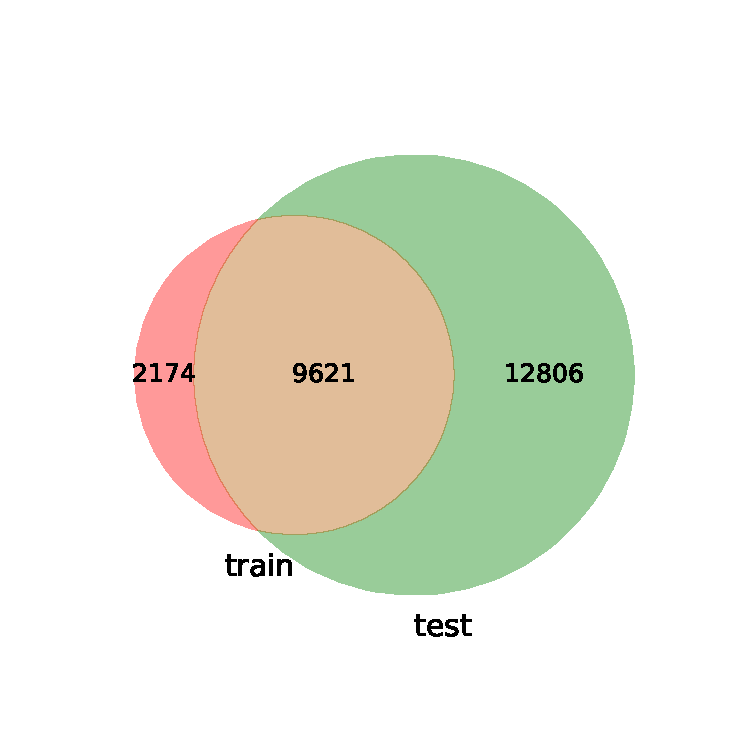
\includegraphics[width=0.4\textwidth]{../Fig/actual_search_term.pdf}}
    \subfigure{\label{Fig:Splitter:b}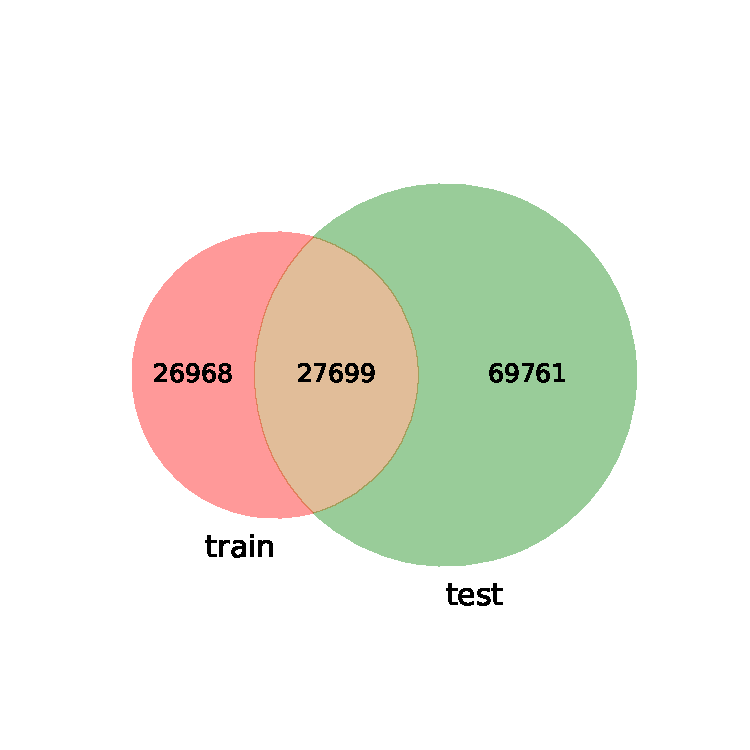
\includegraphics[width=0.4\textwidth]{../Fig/actual_product_uid.pdf}}\vspace{-1cm}\\
    \subfigure{\label{Fig:Splitter:c}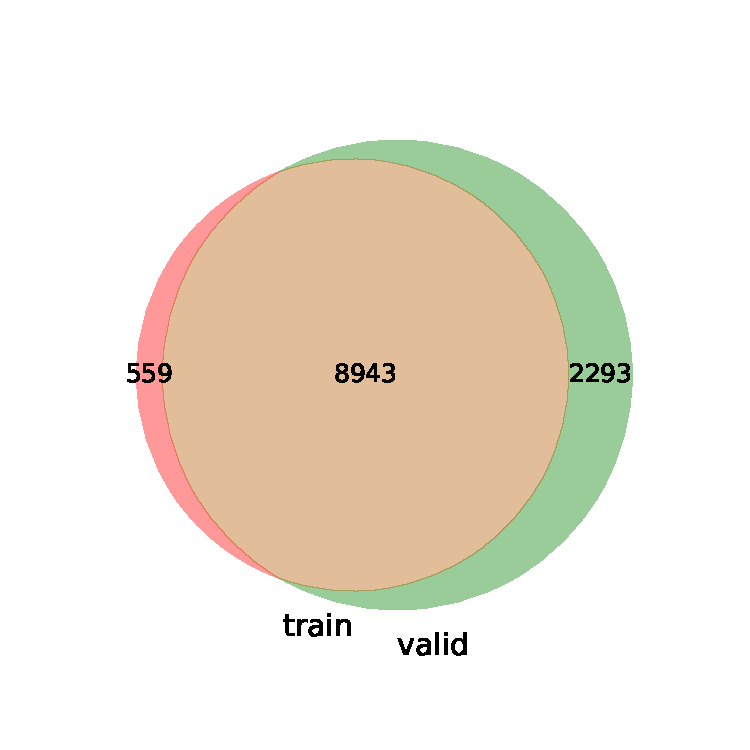
\includegraphics[width=0.4\textwidth]{../Fig/naive_search_term.pdf}}
    \subfigure{\label{Fig:Splitter:d}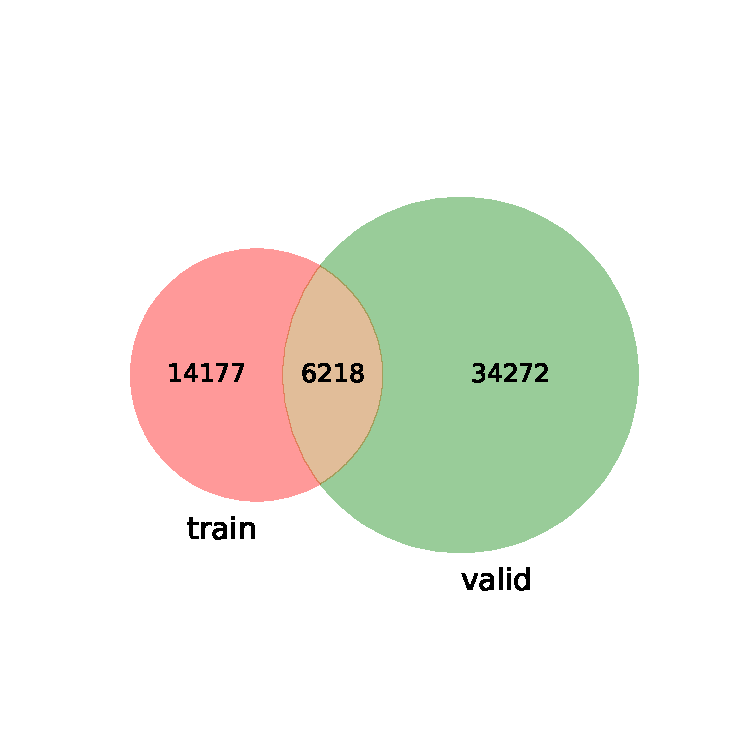
\includegraphics[width=0.4\textwidth]{../Fig/naive_product_uid.pdf}}\vspace{-1cm}\\
    \subfigure{\label{Fig:Splitter:e}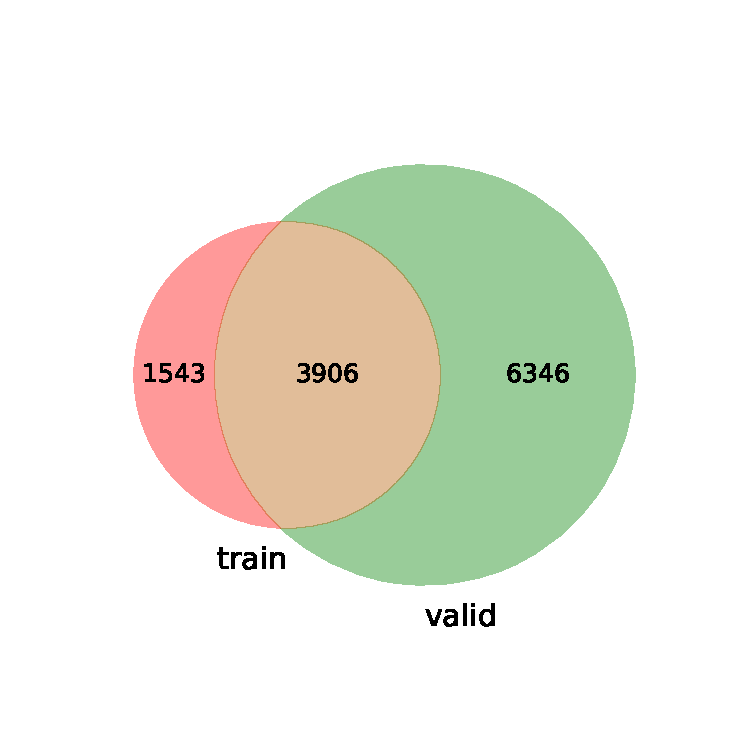
\includegraphics[width=0.4\textwidth]{../Fig/proposed_search_term.pdf}}
    \subfigure{\label{Fig:Splitter:f}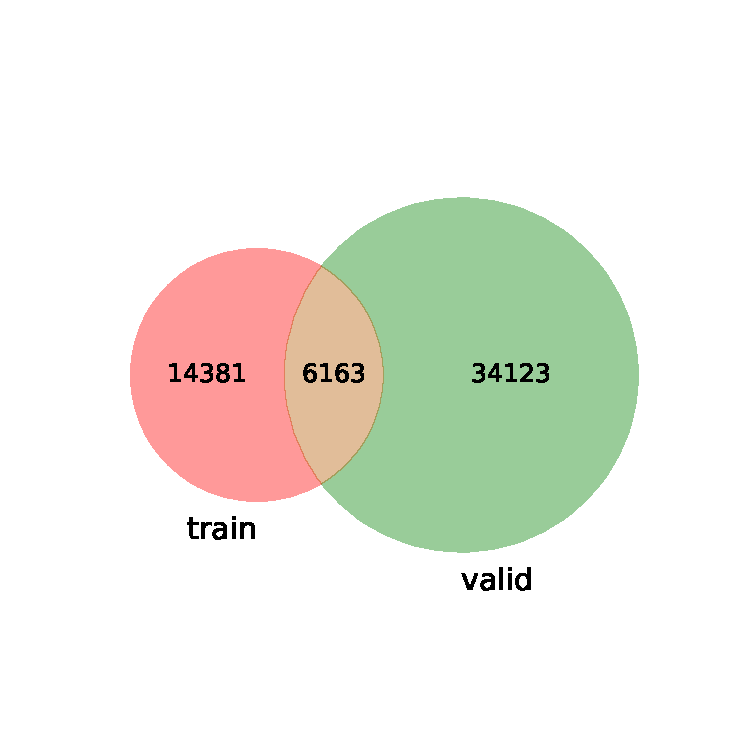
\includegraphics[width=0.4\textwidth]{../Fig/proposed_product_uid.pdf}}
    \caption{Comparison of different splits on search\_term (left column) and product\_uid (right column). From top to bottom, shown are actual train/test split, naive 0.69 : 0.31 random shuffle split, and the proposed split.}
    \label{Fig:Splitter}
\end{figure*}

\begin{figure}
  \centering
  % Requires \usepackage{graphicx}
  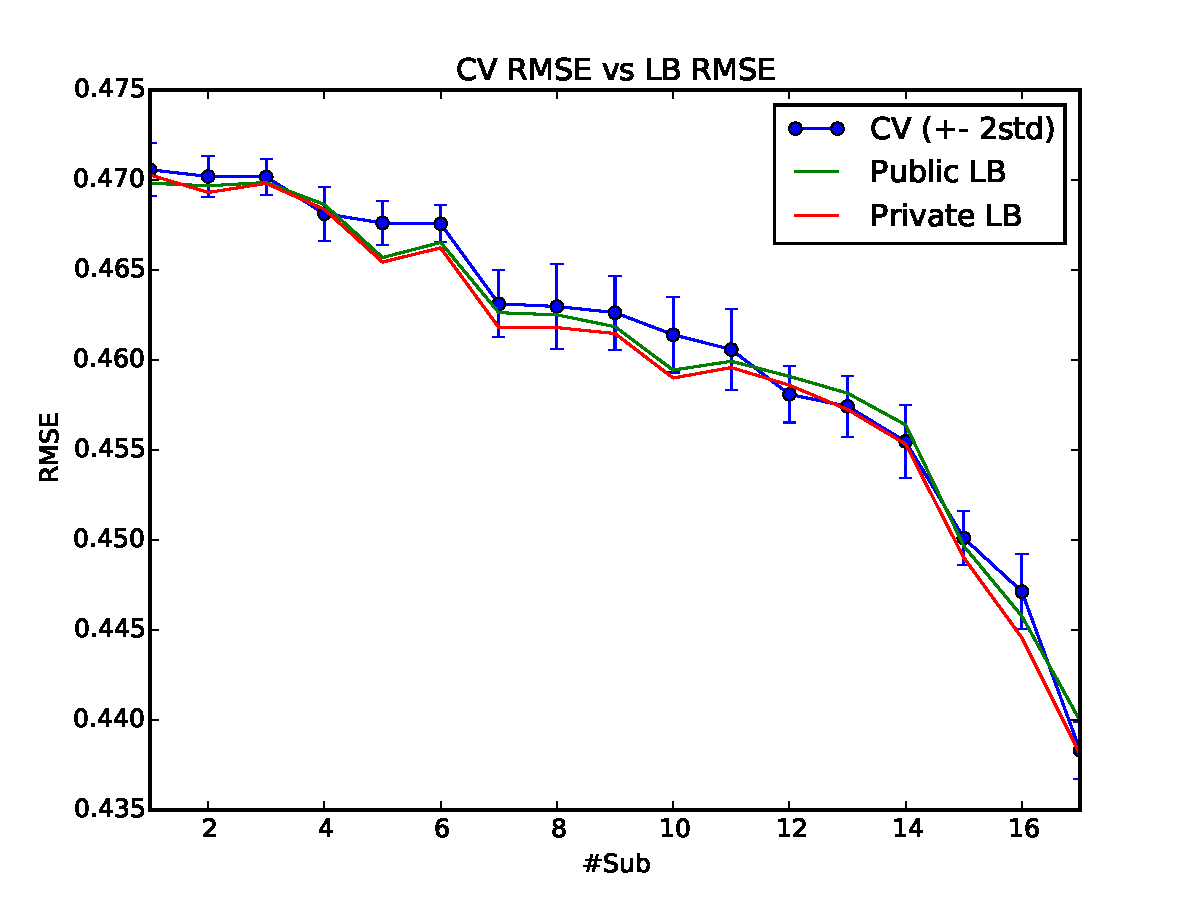
\includegraphics[width=0.75\textwidth]{../Fig/CV_LB_Chenglong.pdf}\\
  \caption{CV RMSE vs LB RMSE for some of Chenglong's submissions.}
  \label{Fig:CV_LB_Chenglong}
\end{figure}

\begin{comment}
The splits I used are in \texttt{./Data/splits}. You can use it as follows:
\begin{verbatim}
# used in python 2
import cPickle as pickle
splits = pickle.load(open("splits_level1_py2.pkl", "rb"))
# 5-run
for trainInd, validInd in splits:
    X_train, X_valid = X[trainInd], X[validInd]
    y_train, y_valid = y[trainInd], y[validInd]
    clf = ...
    clf.fit(X_train, y_train)
    ...
\end{verbatim}

Note that level 1 splits are generated using the whole training data, while level 2 splits using only the corresponding validation data in level 1 split. Similarly, we generate level 3 splits using only the validation data in level 2 split. \textcolor{red}{This is so as to avoid leakage when building stacking models}. Please see \texttt{splitter.py} for how we generate all the splits.
\end{comment}

\subsubsection{Learners}
The learners we used are listed in \ref{tab:Learners_Chenglong}.
\begin{table}[t]
\centering
\caption{Learners of Chenglong}
    \label{tab:Learners_Chenglong}
\begin{tabular}{|c|c|c|}
\hline
Package   & Model & Module\\
\hline\hline
xgboost & XGBoostRegressor & utils.xgb\_utils\\ \hline
\multirow{7}*{sklearn} & GradientBoostingRegressor & \\ \cline{2-3}
  & AdaBoostRegressor & utils.skl\_utils\\ \cline{2-3}
  & ExtraTreesRegressor & \\ \cline{2-3}
  & RandomForestRegressor & \\ \cline{2-3}
  & LinearSVR & utils.skl\_utils\\ \cline{2-3}
  & Ridge & \\ \cline{2-3}
  & Lasso & \\ \hline
keras & KerasDNNRegressor & utils.keras\_utils\\ \hline
rgf & RGFRegressor & utils.rgf\_utils\\ \hline
\end{tabular}
\end{table}

\subsubsection{Base Models}
We build base models with the above learners on various feature subsets. In most of the case, we use correlation to the relevance target as a judgement to include feature into model building or not. In specific, we only consider those features with a correlation higher than a threshold e.g., 0.05. This strategy might be way too simple. Other alternative choices may include using the feature importance returned by GBDT or RF, greedy forward/backward feature selection etc.

\subsubsection{Ensembling}
As first, we mainly focused on using (extreme) ensemble selection which is also used in CrowdFlower. While it still improves the performance of single models, it becomes very time consuming to generate an ensemble as the model library becoming larger and larger. On the other side, since the evaluation metric of the HomeDepot competition is RMSE (which can be directly optimized using gradient method), ensemble selection doesn't offer much edge over simple linear blending and stacking. So we turn to stacking eventually. One notable advantage of stacking is that, besides using the predictions from base models as features, we can also include other meta features, e.g., features used to build base models.



\subsection{Igor\&Kostia's Part}
\subsubsection{Cross Validation}

Throughout the competition we used \emph{StratifiedShuffleSplit} with $\text{test\_size}=0.65$. The idea was to mimic the split between train and test (the test accounts for $69\%$ of the total observations). Such a split gave us a consistent gap between our CV and LB: $\text{LB RMSE} - \text{CV RMSE} \approx 0.002$.

But for our ensembling we wanted that each observation be proportionally present in the training and validation sets, which can not be guaranteed by StratifiedShuffleSplit for any finite number of splits. That is why for ensembling we switched to \emph{StratifiedKFold} with $k=3$ and used only one part for training and two parts for validation, thus implementing the Chenglong's approach for CrowdFlower \cite{CrowdFlower_1st}.


\subsubsection{Learners and Models}
The list of our learners is presented in table \ref{tab:Learners_IandK}.

We found it beneficial to run xgboost as a base model for \emph{BaggingRegressor}. This combination improved RMSE by $0.001$ \ldots $0.002$ (we used $\text{n\_estimators}=10$). For any other our model \emph{BaggingRegressor} would not improve performance.

We built several models on different feature sets and with different parameters. To reduce the number of features, we combined the following approaches:
\begin{itemize}
\item Generated feature importances from our benchmark \emph{GradientBoostingRegressor} model and kept features only above certain importance threshhold.
\item Removed highly correlated features.
\end{itemize}

\begin{table}[t]
\centering
\caption{Learners of Igor\&Kostia}
    \label{tab:Learners_IandK}
\begin{tabular}{|c|c|c|}
\hline
Package   & Model & File\\
\hline\hline
\multirow{2}*{xgboost, sklearn} & \multirow{2}*{BaggingRegressor(XGBoostRegressor())} & generate\_models.py \\ && generate\_model\_wo\_google.py \\ \hline
\multirow{4}*{sklearn} & GradientBoostingRegressor & \multirow{4}*{generate\_models.py} \\ \cline{2-2}
  & ExtraTreesRegressor & \\ \cline{2-2}
  & RandomForestRegressor & \\ \cline{2-2}
  & SVR & \\  \hline
\end{tabular}
\end{table}
\subsubsection{Ensembling}
As an output from the modelling steps we had prediction for validation set and test set. We used linear regression on predictions for validation set to find optimal coefficients for our ensemble and then calculated ensemble predictions for the test set.

\subsubsection{Ensembling2}
Also we would like to describe another ensemble which we use for the final predictions.
This ensemble slightly improved our private LB score from 0.43723 to 0.43704 and has some positive and negative sides. The biggest problem was a skyrocketing gap between CV and LB due to poor cross validation split (\emph{StratifedKFold} with $k = 3$ and two parts used for training and one part used for validation and split was not stable). Nevertheless, we think this ensemble has some interesting ideas and could perform better with the correct split method.

Algorithm description step by step:

\textbf{Level 1 stages} (\texttt{ensemble\_script\_random\_version.py}):
\begin{itemize}
\item[1.] Select list of models for level 1.
\item[2.] Randomly split all features into two subset (first and second part).
\item[3.] Fit and make predictions for each model and each part of features 4 times: 3 for validation and 1 for test (here we use \emph{StratifedKFold} with $k = 3$).
\item[4.] Repeat steps 2 and 3 if computation capacity is available (it requires a lot of time).
\end{itemize}

\textbf{Level 2 stages} (\texttt{model\_selecting.py}):
\begin{itemize}
\item[5.] Use \emph{StratifedKFold} split with $k \geq 5$ for validation predictions of models on level 1. $k-1$ parts are used for fitting level 2 models and 1 part is used for validation.
\item[6.] Only some of the generated models are beneficial to the ensemble. Now we need to identify the list of 'good' models. Start with the empty list.
\item[7.] Add the best (by its validation RMSE) model from level 1 to 'good model list'.
\item[8.] For each level 1 prediction which is not yet in 'good model list', fit level 2 model on the model predictions and predictions from models in 'good model list'. Add that model to 'good model list'  which provides the largest reduction to the ensemble RMSE (We use linear regression/ridge regression as level 2 model).
\item[9.] Repeat 8 while the ensemble RMSE is improving.
\end{itemize}

Advantages of this algorithm are:
\begin{itemize}
\item random feature's subsets are good source of variation which improves the ensemble performance;
\item greedy selection of models for level 2 performs better on LB than the straightforward ensembling of all available level 1 models;
\item the solution can be well automated without any 'hand tuning' or other human intervention (we still need to define the model list for the first step).
\end{itemize}

Disadvantages:
\begin{itemize}
\item  in our case inferior split lead to overfitting on level 2.
\end{itemize}


\subsection{Final Blend}
\label{subsec:final_blend_description}
So, we had two ensembles prepared using different methodologies. We observed that our ensembles behave differently in different parts of the datasets ($\text{part}_1$:  $\text{id} \leq 163700$,  $\text{part}_2$:  $163700<\text{id} \leq 221473$,
$\text{part}_3$:  $\text{id} > 221473$  on  Fig.~\ref{Fig:ensembles_performance}  and other figures in Appendix).  Since we observed regular patterns in the data as well (see Figs.~\ref{Fig:replaced_with_Google}-\ref{Fig:query_with}), we thought that one of the ensembles might be especially prone to overfitting in some parts. So, while blending our ensembles for final submissions, we made different bets assuming that in some parts one of the models would behave much worse in private than in public.

Our two final submission were produced with the weights from Table \ref{tab:weights_final}. They scored the same $0.43271$ on the private leaderboard.

It should be noted that the organizers  \href{https://www.kaggle.com/c/home-depot-product-search-relevance/forums/t/20491/last-20k-rows/117311}{included ``poisoned" test data} (representing $33\%$ of the test set) to discourage hand labeling. In fact, the $\text{part}_3$ was totally formed of poisoned data which was not scored neither in public nor in private.

\begin{table}[t]
\centering
\caption{Weights for the Two Final Submissions}
    \label{tab:weights_final}
\begin{tabular}{|c|c|c|c|c|}
\hline
 & Weight Chenglong                                   & Weight Chenglong        & \multirow{2}*{Public RMSE} & \multirow{2}*{Private RMSE}\\
& for $\text{part}_1$ and $\text{part}_2$ & for $\text{part}_3$    & & \\
\hline\hline
Submission 1 & 0.75 & 0.8 & 0.43443 & 0.43271 \\ \hline
Submission 2 & 0.6 & 0.3 & 0.43433 & 0.43271 \\ \hline
\end{tabular}
Note: The weights for Chenglong and Igor\&Kostia add up to $1$.
\end{table}





\begin{comment}
\newpage
\subsection{Training Level 1 Models}
\begin{verbatim}
# used in python 2
import cPickle as pickle

splits_l1 = pickle.load(open("splits_level1_py2.pkl", "rb"))
models_l1 = Ridge
RMSE_l1 = np.zeros((len(splits_l1)))
y_test_l1 = np.zeros((X_test.shape[0]))

for i, (trainInd_l1, validInd_l1) in enumerate(splits_l1):
    #------------ Level 1 ----------------
    X_train_l1, X_valid_l1 = X[trainInd_l1], X[validInd_l1]
    y_train_l1, y_valid_l1 = y[trainInd_l1], y[validInd_l1]
    clf.fit(X_train_l1, y_train_l1)
    y_pred_l1 = clf.predict(X_valid_l1)
    RMSE_l1[i] = rmse(y_valid_l1, y_pred_l1)
    if i == 0:
        ## refit (only need to run once)
        clf.fit(X, y)
        y_test_l1 = clf.predict(X_test)

## level 1 CV
print(np.mean(RMSE_L1))
print(np.std(RMSE_L1))

## final submission
y_test_l1

\end{verbatim}







\newpage
\subsection{Training Level 2 Models}
\begin{verbatim}
# used in python 2
import cPickle as pickle

splits_l1 = pickle.load(open("splits_level1_py2.pkl", "rb"))
split2_l2 = pickle.load(open("splits_level2_py2.pkl", "rb"))
models_l1 = [Ridge, RandomForestRegressor, GradientBoostingRegressor]
models_l2 = Ridge
RMSE_l1 = np.zeros((len(splits_l1), len(models_l1)))
RMSE_l2 = np.zeros((len(splits_l2)))
y_test_l1 = np.zeros((X_test.shape[0], len(models_l1)))
y_test_l2 = np.zeros((X_test.shape[0], len(splits_l1)))

for i, (trainInd_l1, validInd_l1) in enumerate(splits_l1):
    #------------ Level 1 ----------------
    X_train_l1, X_valid_l1 = X[trainInd_l1], X[validInd_l1]
    y_train_l1, y_valid_l1 = y[trainInd_l1], y[validInd_l1]
    y_pred_l1 = np.zeros((len(validInd_l1), len(models_l1)))
    for j,clf in enumerate(models_l1):
        ## CV
        clf.fit(X_train_l1, y_train_l1)
        y_pred_l1[:,j] = clf.predict(X_valid_l1)
        RMSE_l1[i,j] = rmse(y_valid_l1, y_pred_l1[:,j])
        if i == 0:
            ## refit (only need to run once)
            clf.fit(X, y)
            y_test_l1[:,j] = clf.predict(X_test)

    #------------ Level 2 ----------------
    ## CV
    # In fact splits_l2[i] is obtained using only validInd_l1
    trainInd_l2, validInd_l2 = splits_l2[i]
    X_train_l2, X_valid_l2 = y_pred_l1[trainInd_l2], y_pred_l1[validInd_l2]
    y_train_l2, y_valid_l2 = y_valid_l1[trainInd_l2], y_valid_l1[validInd_l2]
    models_l2.fit(X_train_l2, y_train_l2)
    y_pred_l2 = models_l2.predict(X_valid_l2)
    RMSE_l2[i] = rmse(y_valid_l2, y_pred_l2)

    ## refit
    # here, I train a model for each run
    # you can also concat y_pred_l1 of each run to a large
    # matrix and only train one model (outside this for-loop)
    models_l2.fit(y_pred_l1, y_valid_l1)
    y_test_l2[:,i] = models_l2.predict(y_test_l1)

## level 1 CV
print(np.mean(RMSE_l1, axis=0))
print(np.std(RMSE_l1, axis=0))

## level 2 CV
print(np.mean(RMSE_l2))
print(np.std(RMSE_l2))

## final submission
# average over 5-run
y_test_l2 = np.mean(y_test_l2, axis=1)

\end{verbatim}
\end{comment}

\section{Code Description}
\subsection{Chenglong's Part}
All the code are in \texttt{./Code/Chenglong}.
\subsubsection{Config}
All the pathes, parameters, and other configurations are set via \texttt{config.py}.
\subsubsection{Data Processing}
\begin{itemize}
\item \texttt{data\_preparer.py}: generate raw dataframe data
\item \texttt{data\_processor.py}: process data
\begin{itemize}
\item a bunck of processing
\item automated spelling correction
\item query expansion
\item extract product name for search\_term and product\_title
\end{itemize}
\item \texttt{google\_spelling\_checker\_dict.py}: contains google spelling correction dictionary from this \href{https://www.kaggle.com/steubk/home-depot-product-search-relevance/fixing-typos}{Kaggle forum post}
\item \texttt{spelling\_checker.py}: home-made spelling checker inspired by Peter Norvig's post\cite{PeterNorvig} (though not used in the final submission)
\end{itemize}
\subsubsection{Feature Generation}
\begin{itemize}
\item \texttt{feature\_base.py}: base class for feature generation, including \texttt{BaseEstimator}, \texttt{StandaloneWrapper} and \texttt{PairwiseWrapper}
\item \texttt{feature\_combiner.py}: combine a bunch of single feature (specified via a feature conf file) into a feature matrix
\item \texttt{feature\_transformer.py}: various feature transformations
\item \texttt{feature\_[basic|distance|doc2vec|...].py}: various feature generators; see \ref{subsec:FeatureExtraction_Chenglong} for details
\item \texttt{embedding\_trainer.py}: script for training word2vec and doc2vec models with the provided data
\item \texttt{get\_feature\_conf\_*.py}: generate feature conf file as input for \texttt{feature\_combiner.py}
\item \texttt{convert\_pkl\_lsa\_to\_csv\_lsa.py}: convert \texttt{.pkl} format LSA features to \texttt{.csv} format for using \texttt{Rtsne} package in R
\item \texttt{convert\_csv\_tsne\_to\_pkl\_tsne.py}: convert \texttt{.csv} format TSNE features to \texttt{.pkl} format
\end{itemize}
\subsubsection{Task}
\begin{itemize}
\item \texttt{task.py}: definitions for
\begin{itemize}
\item learner \& ensemble learner
\item feature \& stacking feature
\item task \& stacking task
\item task optimizer
\end{itemize}
It is also the wrapper for running various tasks with various features and various learners.
\item \texttt{model\_param\_space.py}: contains parameter searching space for various learners
\item \texttt{run\_[test\_ridge|test\_xgb|stacking\_ridge].py}: some scripts for running the following procedure in one shot
\begin{itemize}
\item generate feature conf
\item generate feature matrix
\item run task
\end{itemize}
This is for accelerating the circle of change-validate-check.
\item \texttt{extreme\_ensemble\_selection.py}: generate submission via extreme ensemble selection
\end{itemize}
\subsubsection{Other}
\begin{itemize}
\item \texttt{run\_data.py}: generate data and features in one shot
\item \texttt{splitter.py}: generate splitter for all the models including 1st, 2nd and 3rd level models
\item \texttt{turing\_test\_converter.py}: convert \texttt{.csv} format dataframe features (from Igor\&Kostia) to \texttt{.pkl} format features
\item \texttt{./utils}: utils for various modules
\begin{itemize}
\item \texttt{dist\_utils.py}: utils for distance computation
\item \texttt{keras\_utils.py}: utils for Keras models
\item ...
\end{itemize}
\end{itemize}



\subsection{Igor\&Kostia's Part}
\label{subsec:code_IandK}
All the code are in \texttt{./Code/Igor\&Kostia}.
\subsubsection{Config}
All the paths  are set via \texttt{config\_IgorKostia.py}.


\subsubsection{Data Processing}
Since the same text processing steps should be performed in order to generate different features, we decided to do all text processing before any feature generation. This approach helped us to calculate the result a few days faster if compared with step-by-step feature generation from the input text files.
\begin{itemize}
\item \texttt{homedepot\_functions.py}: contains many functions used for text processing and in some other steps.
\item  \texttt{google\_dict.py}  contains google spelling correction dictionary from \cite{Google_dict}.
\item \texttt{text\_processing.py} and  \texttt{text\_processing\_wo\_google.py} implement the same text processing steps, except the latter file does not uses replacement from the Google dictionary from the forum.
\end{itemize}
\subsubsection{Feature Generation}
\begin{itemize}
\item \texttt{feature\_extraction1.py} and \texttt{feature\_extraction1\_wo\_google.py}: the same logic, but input produced with or without Google dictionary. These files generate basic features, some distance features, brand and material features, some TFIDF features, WordNet similarity features, query expansion features and dummies (see section \ref{subsec:Features_IandK})
\item \texttt{grams\_and\_terms\_features.py}: generates a part of the distance features (see section \ref{subsubsec:Distance_Features_IandK}).
\item \texttt{dld\_features.py}: generates the final part of the distance features  (see section \ref{subsubsec:Distance_Features_IandK}), namely involving the Damerau-Levenshtein distances.
\item \texttt{word2vec.py} and \texttt{word2vec\_without\_google\_dict.py}: generate word2vec features  (see section \ref{subsubsec:word2vec_IandK}).
\end{itemize}

\subsubsection{Modelling}
\begin{itemize}
\item \texttt{generate\_feature\_importances.py}: supplies all generated feature into our benchmark \emph{GradientBoostingRegressor} model and gets the list of feature importances.
\item \texttt{generate\_models.py} and \texttt{generate\_model\_wo\_google.py}: create appropriate feature lists, fit a number of models on those features, generate validation results and prediction results for test dataset.
\item \texttt{generate\_ensemble\_output\_from\_models.py}: reads the output from the previous step and generates ensemble submission.
\end{itemize}

\subsubsection{Modelling2}
This is the necessary code to reproduce our results, although this part is not crucial for our performance because of inferior cross-validation split (\emph{StratifiedKFold} with $k=3$, two part used for training and one for validation). However, we tried a few advanced techniques for model selection here, which might be promising.
\begin{itemize}
\item \texttt{ensemble\_script\_random\_version.py}: selects random feature subsets and generates validation and test predictions using a different split.
\item \texttt{ensemble\_script\_imitation\_version.py}: reproduces the output from previous step used in our submission.
\item \texttt{model\_selecting.py}: selects models and generates ensemble submission.
\end{itemize}




\section{Simple Features and Methods}
\label{sec:simplified}
As suggested by the Kaggle documentation template, we generated a model with only 10 features  and got private RMSE of $0.44949$ ( 31st place on the leaderboard). Please see
section \ref{subsec:Results_description} to compare this with our best submissions.

Feature importances for the simplified model are shown on Fig.~\ref{Fig:feature_importance_simplified_IandK}

\begin{figure}
  \centering
  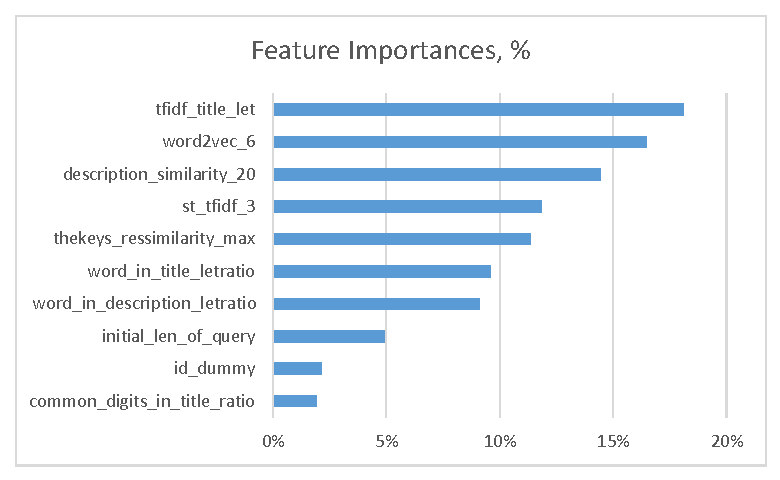
\includegraphics[width=0.7\textwidth]{../Fig/plot_feature_importances_simplified_model.pdf}\\
  \caption{Feature importances for simplified model with 10 features (Igor\&Kostia).}
  \label{Fig:feature_importance_simplified_IandK}
Note: \textbf{word2vec\_6} was calculated as \emph{n\_similarity()} between stemmed search term and stemmed product title.
\textbf{description\_similarity\_20} is the feature generated from query expansion to 20 most common words (section \ref{subsubsec:queryexpansion_IandK}). \textbf{st\_tfidf\_3} is just the number of rows in the dataset with a particular search term.
\end{figure}



\section{Additional Comments and Observations}
Some interesting insights we got during the competition:
\begin{itemize}
\item Spelling correction/synonyms replacement/text cleaning are very useful for searching query relevance prediction as also revealed in CrowdFlower.
\item In this competition, it is quite hard to improve the score via ensemble and stacking. To get the most out of ensemble and stacking, one should really focus on introducing diversity. To that goal, try various text processing, various feature subsets, and various learners. Team merging also contribute a lot of diversity!
\item That said, know how to separate the effect of improved algorithm from the effect of increased diversity. Careful experiments are necessary. If some clear and effective solution does not work as well as your old models, do not discard it until you compare both approaches in the same conditions.
\item Keep a clean and scalable codebase. Keep track/log of the change you have made, especially how you create those massive crazy ensemble submission.
\item Set up an appropriate and reliable CV framework. This allows to try various local optimizations on the features \& models and getting feedback without the need to submit them. This is important for accelerating the change-validate-check cycle.
\item After team merging, we have spent some effort on figure out the best way to ensemble our results. Due to the fact that we do not use the same CV split, we cannot run something like 2nd level stacking. In the end, we go with the simple weight average method. We might have better results if we have merged early on. But that might also reduce the diversity of our models, which might be harmful for ensemble as well. But who knows.
\item We were thinking that features measuring how close is the \{ length, width, height, depth, volume, weight, color\} of the product in search\_term and product\_title would be predictive. However, we did not manage to spare out some time to explore these things.
\end{itemize}












\section{Acknowledgement}
We would like to thank the DMLC team for developing the great machine learning package xgboost, Fran\c{c}ois Chollet for developing package keras, James Bergstra for developing package hyperopt, Radim {\v R}eh{\r u}{\v r}ek for developing package gensim. We would also like to thank the Kaggle team and Homedepot for organizing this competition.

Igor would like to thank his wife Anastasiia for her support and inspiration during this competition.




\bibliographystyle{plain}
\bibliography{reference,reference2}








\begin{appendices}
\newpage

\section{Model Execution Time}

\begin{itemize}
\item \textbf{What software did you use for training and prediction?}\\
Please see section Appendix \ref{sec:dependencies}.

\item \textbf{What hardware (CPUS spec, number of CPU cores, memory)?}\\
Chenglong: 8-Core i7-4790 3.60GHz, 16GB RAM running Windows; 16-Core E5520 2.27GHz, 36GB RAM running Linux;

Igor\&Kostia: 4-Core i5 2.8 GHz, 16GB RAM running Windows.

\item \textbf{How long does it take to train your model?}\\
Chenglong: Feature generation part takes $1\sim 2$ days to finish, depending on the computational power. This is for Chenglong's feature alone. Prediction and training for the best single model from Chenglong takes a few minutes to run. To reproduce Chenglong's best ensemble submission which relies on a few hundreds of 1st level models, it will take a few days. The \texttt{AdaBoostRegressor}, \texttt{GradientBoostingRegressor}, and \texttt{RGFRegressor} are the most time consuming models to train. But including a few of them is useful for the ensemble.

Igor\&Kostia: Text processing and feature generation takes a few days.  Prediction and training for a single model can take from $\sim 5$ minutes (xgboost) to $\sim 5$ hours (SVR).

\item \textbf{How long does it take to train the simplified model (referenced in section \ref{sec:simplified})?}\\
We did not try to generate the used features very fast. Training and prediction takes a few seconds.

\end{itemize}





\section{Dependencies}
\label{sec:dependencies}
\subsection{Chenglong's Part}
\label{subsec:Dependencies_Chenglong}
\subsubsection{Python}
We used Python 3.5.1 and modules comes with \href{https://repo.continuum.io/archive/Anaconda3-2.4.1-Linux-x86\_64.sh}{Anaconda 2.4.1 (64-bit)}. In addition, we also used the following libraries and modules:
\begin{itemize}
\item \href{https://github.com/piskvorky/gensim/archive/0.12.4.tar.gz}{gensim 0.12.4}
\item \href{https://github.com/hyperopt/hyperopt}{hyperopt 0.0.3.dev}
\item \href{https://github.com/fchollet/keras/archive/0.3.2.tar.gz}{keras 0.3.2}
\item \href{https://pypi.python.org/pypi/matplotlib-venn}{matplotlib-venn 0.11.3}
\item \href{https://pypi.python.org/pypi/python-Levenshtein/0.12.0}{python-Levenshtein 0.12.0}
\item \href{https://pypi.python.org/pypi/regex}{regex 2.4.85}
\item \href{https://github.com/dmlc/xgboost/archive/v0.40.tar.gz}{xgboost 0.4}
\end{itemize}
\subsubsection{R}
We used the following packages installed via \texttt{install.packages()}:
\begin{itemize}
\item data.table
\item Rtsne
\end{itemize}
\subsubsection{Other}
We used the following thirdparty packages:
\begin{itemize}
\item \href{http://stat.rutgers.edu/home/tzhang/software/rgf/rgf1.2.zip}{rgf 1.2}
\end{itemize}



\subsection{Igor\&Kostia's Part}
\label{subsec:Dependencies_IandK}
\subsubsection{Python}
We used Python 2.7.11  on Windows platform and modules comes with Anaconda 2.4.0 (64-bit), including:
\begin{itemize}
\item scikit-learn 0.17.1
\item numpy 1.10.1
\item pandas 0.17.0
\item re 2.2.1
\item matplotlib 1.4.3
\item scipy 0.16.0
\end{itemize}

In addition, we also used the following libraries and modules:
\begin{itemize}
\item NLTK 3.1 (use \emph{nltk.download()} command)
\item \href{https://github.com/piskvorky/gensim/archive/0.12.2.tar.gz}{gensim 0.12.2}
\item \href{https://github.com/dmlc/xgboost/archive/v0.40.tar.gz}{xgboost 0.4}
\end{itemize}

Some descriptive analysis was also done in Excel 2007 and Excel 2010.




\section{How To Generate the Solution (aka README file)}
\subsection{Chenglong's Part}
Before proceeding, one should place all the data from the \href{https://www.kaggle.com/c/home-depot-product-search-relevance/dat}{competition website} into folder \texttt{./Data}. Note that in the following, all the commands and scripts are executed and run in directory \texttt{./Code/Chenglong}.

\subsubsection{Step 1. Install Dependencies}
Make sure you have installed all the dependencies listed in \ref{subsec:Dependencies_Chenglong}.

\subsubsection{Step 2. Prepare External Data}
\textbf{1. Pre-trained Word2Vec Model}\\
We used pre-trained Word2Vec models listed in this \href{https://github.com/3Top/word2vec-api}{Github repo}. In specific:
\begin{itemize}
\item \href{https://drive.google.com/file/d/0B7XkCwpI5KDYNlNUTTlSS21pQmM/}{Google News}
\item \href{http://nlp.stanford.edu/data/glove.6B.zip}{Wikipedia+Gigaword 5}
\end{itemize}
We used glove-gensim\cite{glove-gensim} to convert GloVe vectors into Word2Vec format for easy usage with Gensim. After that, put all the models in the corresponding directory (see \texttt{config.py} for detail).\\
\textbf{2. Other}\\
We also used the following external data:
\begin{itemize}
\item Color data from this \href{https://www.kaggle.com/c/home-depot-product-search-relevance/forums/t/18967/data-preparation}{Kaggle forum post}, i.e., \texttt{./Data/dict/color\_data.py}.
\item Google spelling correction dictionary from this \href{https://www.kaggle.com/steubk/home-depot-product-search-relevance/fixing-typos}{Kaggle forum post}, i.e.,\\\texttt{google\_spelling\_checker\_dict.py}.
\item Home-made word replacement dictionary, i.e., \texttt{./Data/dict/word\_replacer.csv}.
\item NLTK corpora and taggers data downloaded using \texttt{nltk.download()}, specifically: \texttt{stopwords.zip}, \texttt{wordnet.zip} and \texttt{maxent\_treebank\_pos\_tagger.zip}.
\end{itemize}

\subsubsection{Step 3. Generate Features}
To generate data and features, one should run \texttt{python run\_data.py}. While we have tried our best to make things as parallelism and efficient as possible, this part might still take $1\sim 2$ days to finish, depending on the computational power. So be patient :)

Note that various text processing are useful for introducing diversity into ensemble. As a matter of fact, one feature set (i.e., \texttt{basic20160313}) from our final solution is generated before the \href{https://www.kaggle.com/steubk/home-depot-product-search-relevance/fixing-typos}{Fixing Typos post}, i.e., not using the Google spelling correction dictionary. Such version of features can be generated by turning off the \texttt{GOOGLE\_CORRECTING\_QUERY} flag in \texttt{config.py}.

After team merging with Igor\&Kostia, we have rebuilt everything from scratch, and most of our models used different subsets of Igor\&Kostia's features. For this reason, you should also need to follow Sec. \ref{subsubsec:README_Igor_Kostia} to generate their features. Since Igor\&Kostia's features are in \texttt{.csv} dataframe format, we provide a converter \texttt{turing\_test\_converter.py} to convert them to the format we use, i.e., \texttt{.pkl}.

\subsubsection{Step 4. Generate Feature Matrix}
In step 3, we have generated a few thousands of features. However, only part of them will be used to build our model. For example, we don't need those features that have very little predictive power (e.g., have very small correlation with the target relevance.) Thus we need to do some feature selection. In our solution, feature selection is enabled via the following two successive steps.\\
\textbf{1. Regex Style Manual Feature Selection}\\
This approach is implemented as \texttt{get\_feature\_conf\_*.py}. The general idea is to include or exclude specific features via \textit{regex} operations of the feature names. For example,
\begin{itemize}
\item one can specify the features that he want to \textbf{include} via the \texttt{MANDATORY\_FEATS} variable, despite of its correlation with the target
\item one can also specify the features that he want to \textbf{exclude} via the \texttt{COMMENT\_OUT\_FEATS} variable, despite of its correlation with the target (\texttt{MANDATORY\_FEATS} has higher priority than \texttt{COMMENT\_OUT\_FEATS}.)
\end{itemize}
The output of this is a feature conf file. For example, after running the following command:\\
\texttt{python get\_feature\_conf\_nonlinear.py -d 10 -o feature\_conf\_nonlinear\_201605010058.py}
we will get a new feature conf \texttt{./conf/feature\_conf\_nonlinear\_201605010058.py} which contains a feature dictionary specifying the features to be included in the following step.

One can play around with \texttt{MANDATORY\_FEATS} and \texttt{COMMENT\_OUT\_FEATS} to generate different feature subset. We have included in \texttt{./conf} a few other feature confs from our final submission. Among them, \texttt{feature\_conf\_nonlinear\_201604210409.py} is used to build the best single model.\\
\textbf{2. Correlation based Feature Selection}\\
With the above generated feature conf, one can combine all the features into a feature matrix via the following command:\\
\texttt{python feature\_combiner.py -l 1 -c feature\_conf\_nonlinear\_201604210409 -n basic\_nonlinear\_201604210409 -t 0.05}

The \texttt{-t 0.05} above is used to enable the correlation base feature selection. In this case, it means: drop any feature that has a correlation coef lower than \texttt{0.05} with the target relevance.

TODO(Chenglong): Explore other feature selection strategies, e.g., greedy forward feature selection (FFS) and greedy backward feature selection (BFS).

\subsubsection{Step 5. Generate Submission}
\label{subsubsec:GenerateSubmission}
\textbf{1. Various Tasks}\\
In our solution, a \texttt{task} is an object composite of a specific \texttt{feature} (e.g., \texttt{basic\_nonlinear\_201604210409}) and a specific \texttt{learner} (e.g., \texttt{XGBoostRegressor} from \href{https://github.com/dmlc/xgboost}{xgboost}. The definitions for \texttt{task}, \texttt{feature} and \texttt{learner} are in \texttt{task.py}.

Take the following command for example.\\
\texttt{python task.py -m single -f basic\_nonlinear\_201604210409 -l reg\_xgb\_tree -e 100}
\begin{itemize}
\item It runs a \texttt{task} with \texttt{feature} \texttt{basic\_nonlinear\_201604210409} and \texttt{learner} \texttt{reg\_xgb\_tree}.
\item The \texttt{task} is optimized with \href{https://github.com/hyperopt/hyperopt}{hyperopt} for 100 evals for searching the best parameters for learner \texttt{reg\_xgb\_tree}.
\item The \texttt{task} performs both CV and final refit. CV in this case has two purposes: 1) guide hyperopt to find the best parameters, and 2) generate predictions for each CV fold for further (2nd and 3rd level) stacking.
\item For all the available learners and the corresponding parameter searching space, please see \texttt{model\_param\_space.py}.
\end{itemize}

During the competition, we have run various tasks (i.e., various features and various learners) to generate a diverse 1st level model library. Please see \texttt{./Log/level1\_models} for all the tasks we have included in our final submission.\\
\textbf{2. Best Single Model}\\
After generating the \texttt{feature} \texttt{basic\_nonlinear\_201604210409} (see step 4 how to generate this), run the following command to generate the best single model:\\
\texttt{python task.py -m single -f basic\_nonlinear\_201604210409 -l reg\_xgb\_tree\_best\_single\_model -e 1}

This should generate a submission with local CV RMSE around $0.438\sim 0.439$ (and private LB RMSE around 0.438).\\
\textbf{3. Best Ensemble Model}\\
After building \textbf{some diverse} 1st level models, run the following command to generate the best ensemble model:\\
\texttt{python run\_stacking\_ridge.py -l 2 -d 0 -t 10 -c 1 -L reg\_ensemble -o}

This should generate a submission with local CV RMSE around 0.436.




\subsection{Igor\&Kostia's Part}
Before proceeding, one should specify correct paths in file \texttt{config\_IgorKostia.py} and place all the data from the \href{https://www.kaggle.com/c/home-depot-product-search-relevance/dat}{competition website} into folder specified by variable \texttt{DATA\_DIR}.  To reproduce our $\text{Ensemble}_B$   from section \ref{subsubsec:generate_submission_IandK}  one should place the used feature sets into folder specified by variable \texttt{FEATURESETS\_DIR}. Note that in the following, all the commands and scripts are executed and run in directory \texttt{./Code/Igor\&Kostia}.

\subsubsection{Step 1. Install Dependencies}
Make sure you have installed all the dependencies listed in \ref{subsec:Dependencies_IandK}.

\subsubsection{Step 2. Text Preprocessing}
We do all text preprocessing before any feature generation and save the results to files. It helped us save a few computing days since the same preprocessing steps are necessary to generate different features.
\begin{itemize}
\item Run \texttt{text\_processing.py};
\item Run  \texttt{text\_processing\_wo\_google.py}
\end{itemize}

The necessary replacement data is loaded automatically from files  \texttt{homedepot\_functions.py} and \texttt{google\_dict.py}.
\subsubsection{Step3. Feature Generation}
\label{subsubsec:README_Igor_Kostia}

We need to run consequently the following files:
\begin{itemize}
\item \texttt{feature\_extraction1.py}.
\item \texttt{grams\_and\_terms\_features.py}.
\item  \texttt{dld\_features.py}.
\item \texttt{word2vec.py}.
\end{itemize}

To generate features without using the Google dictionary, we also need to run:
\begin{itemize}
\item \texttt{feature\_extraction1\_wo\_google.py}.
\item \texttt{word2vec\_without\_google\_dict.py}.
\end{itemize}

As a result, we will have a few csv files with the necessary features for model building. Please see more information in section \ref{subsec:code_IandK}.

\subsubsection{Step 4. Generate Benchmark Model with Feature Importances}
\begin{itemize}
\item Run \texttt{generate\_feature\_importances.py}.
\end{itemize}

\subsubsection{Step 5. Generate Submission File}
\label{subsubsec:generate_submission_IandK}
One part of the ensemble ($\text{Ensemble}_A$) is generated from the following code:
\begin{itemize}
\item \texttt{generate\_models.py}.
\item \texttt{generate\_model\_wo\_google.py}.
\item \texttt{generate\_ensemble\_output\_from\_models.py}.
\end{itemize}

To get the other part ($\text{Ensemble}_B$), we need to run these files:
\begin{itemize}
\item \texttt{ensemble\_script\_imitation\_version.py} (It just reproduces the selection of random features generated from \texttt{ensemble\_script\_random\_version.py}. You do not need to run \texttt{ensemble\_script\_random\_version.py} again).
\item \texttt{model\_selecting.py}.
\end{itemize}

These two parts can be generated in parallel. Our final submission from Igor\&Kostia was then prodused in Excel as:
$$\text{Output}=0.75\times \text{Ensemble}_A+ 0.25\times \text{Ensemble}_B$$


\subsection{Blending Two Ensembles into the Final Submissions}
This step was done in Excel using the weights described in section \ref{subsec:final_blend_description}.


\newpage
\section{Some charts}
\begin{figure}[h]
  \centering
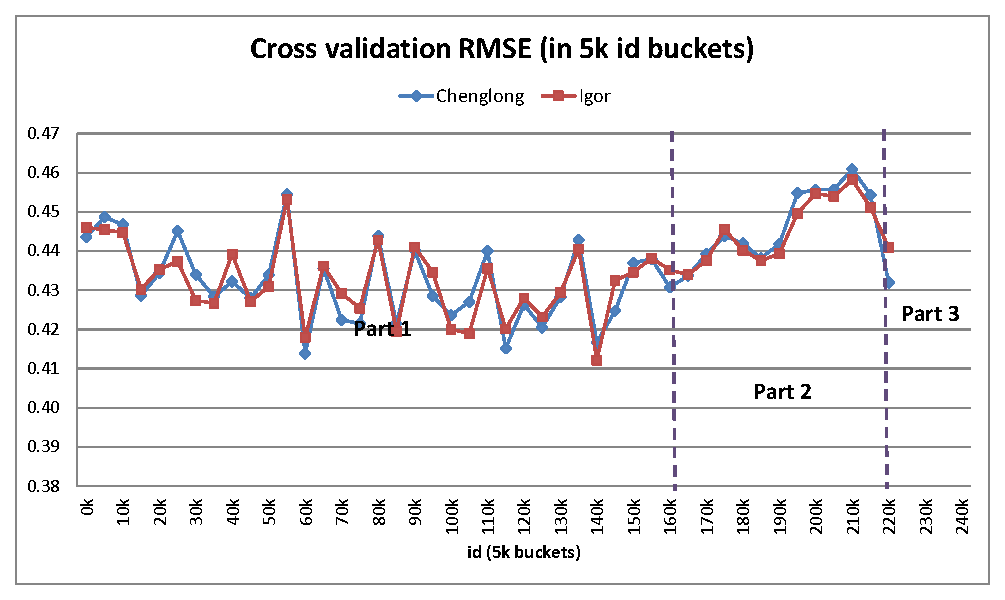
\includegraphics[width=0.7\textwidth]{../Fig/plot_ensembles_performance.pdf}\\
  \caption{Cross validation RMSE of ensembles.}
  \label{Fig:ensembles_performance}
  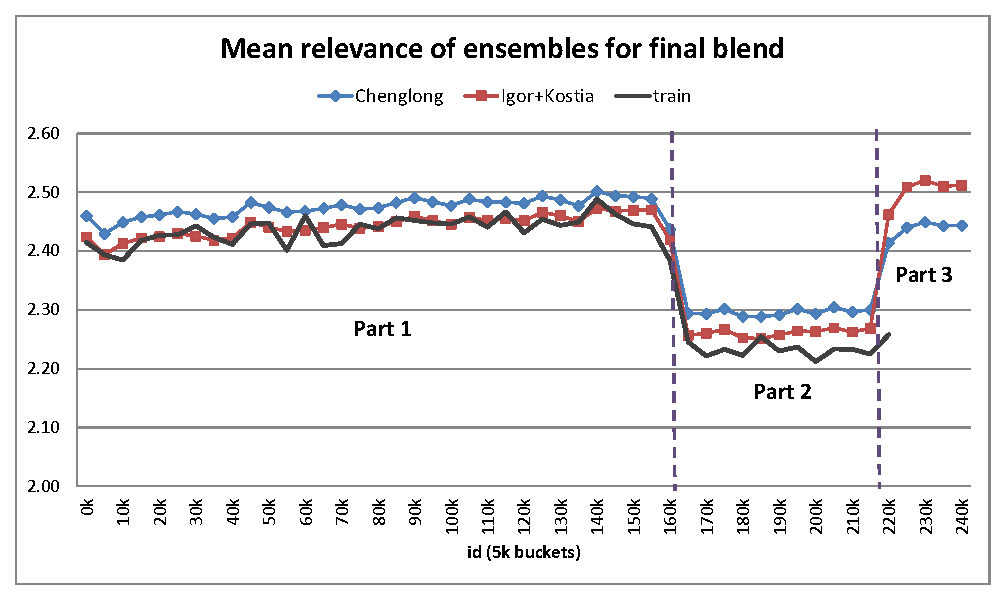
\includegraphics[width=0.7\textwidth]{../Fig/plot_ensembles_means.pdf}\\
  \caption{Mean relevance of ensembles for final blend.}
  \label{Fig:ensembles_means}
\end{figure}

\begin{figure}
  \centering
  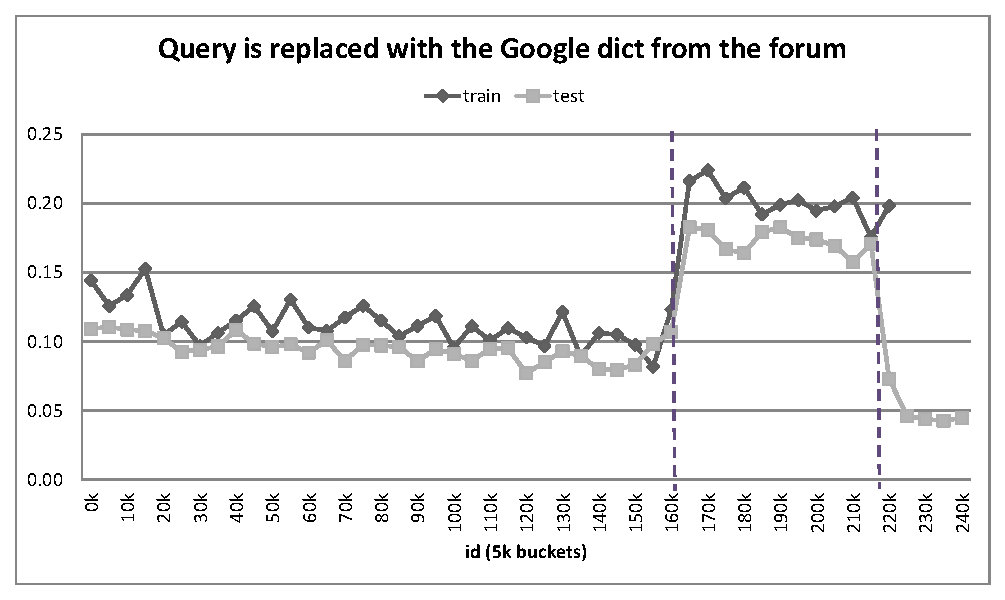
\includegraphics[width=0.7\textwidth]{../Fig/plot_replaced_with_Google.pdf}\\
  \caption{Query is replaced with the Google dictionary from the forum. (Note the difference between train and test).}
  \label{Fig:replaced_with_Google}
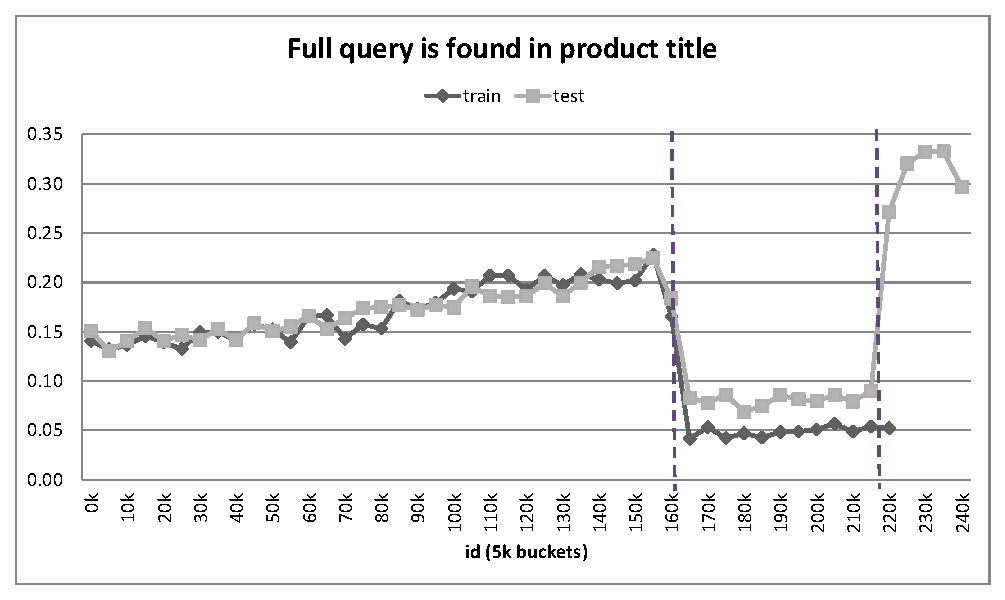
\includegraphics[width=0.7\textwidth]{../Fig/plot_full_query_in_title.pdf}\\
  \caption{Full query is found in product title.}
  \label{Fig:full_query_in_title}
\end{figure}

\begin{figure}
  \centering
  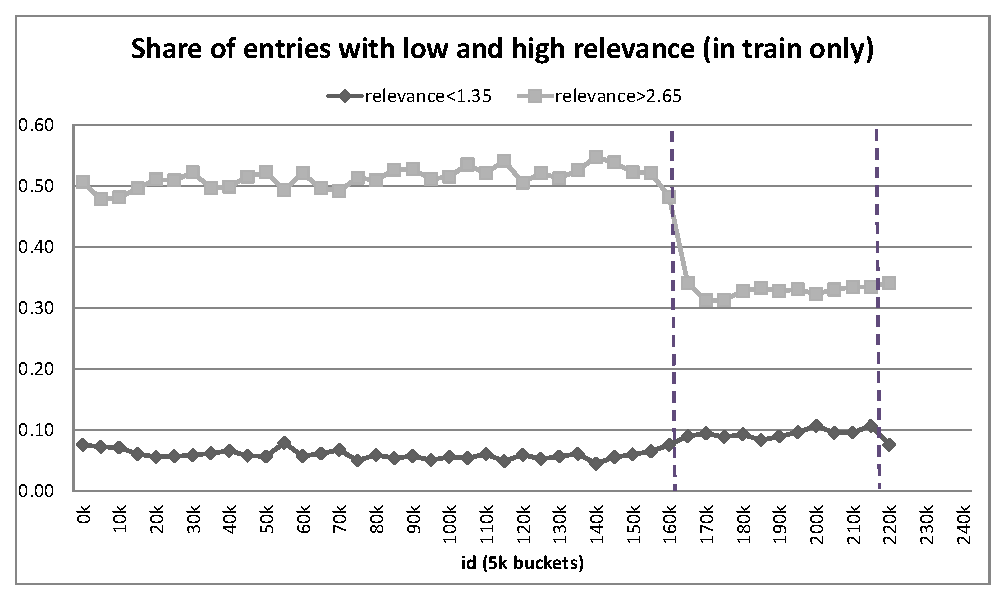
\includegraphics[width=0.7\textwidth]{../Fig/plot_high_vs_low_relevance.pdf}\\
  \caption{Share of entries with low and high relevance (in train only).}
  \label{Fig:high_vs_low_relevance}
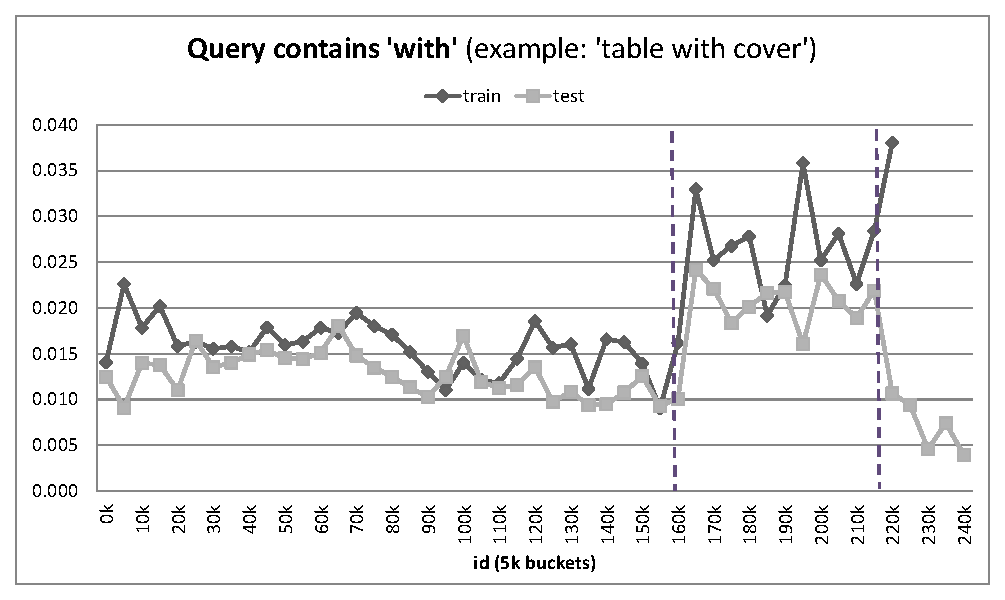
\includegraphics[width=0.7\textwidth]{../Fig/plot_query_with.pdf}\\
  \caption{Query contains \emph{'with'} (example: \emph{'table with cover'}).}
  \label{Fig:query_with}
\end{figure}


\end{appendices}

\end{document}
